\documentclass[../MasterThesis.tex]{subfiles}
\graphicspath{ {./assets/images/} }


%----------------------------------------------------------------------------
%----------------------------------------------------------------------------

\begin{document}
	
	
	
%
%
%
%
%=======================================================================================================
%
%
%
%
%=======================================================================================================
% CHAPTER: DESIGN AND IMPLEMENTATION
%=======================================================================================================
\newpage
\section{Design and Implementation} \label{section:designandimplementation}

In this Chapter, the system architecture and the implementation is explained. First a brief overview over the architecture is given in Section~\ref{subsection:architecturedesign} and then the frontend and backend are described in more detail in Section~\ref{subsection:accuratevideo} and Section~\ref{subsection:jit-webrtc}.
For the application of a Melt filter, different filters were compared to select the most suitable option in Section~\ref{subsection:meltfilter}.





%-------------------------------------------------------------------------------------------------------
\subsection{Architecture Design} \label{subsection:architecturedesign}
% Describe the overall architecture of the system.

%Provide an overview of the system architecture and design. This could include high-level diagrams, such as system flowcharts or architecture diagrams, to illustrate the structure of the software.
%Introduce the existing codebase and its components. Briefly describe the major modules or sections of the code.
%Explain the design decisions made during the development process. Discuss the rationale behind the chosen architecture, programming languages, and frameworks.
%Present any relevant design patterns or paradigms applied in the codebase.
%Provide a detailed description of how the existing code works. This involves explaining the functionality of key modules or sections, the flow of data, and how different components interact.
%If applicable, discuss any algorithms or data structures implemented in the codebase.
%Highlight any challenges or considerations encountered during the implementation phase and how they were addressed.
%Include code snippets, illustrations, or diagrams to enhance the understanding of your codebase.

The system consists of four components: the frontend (browser), Melt, \texttt{main.py}, and a session service. The frontend is described in Section~\ref{subsection:accuratevideo} and the backend (Melt, \texttt{main.py} and session service) will be described in more detail in Section~\ref{subsection:jit-webrtc}. 
In those Sections, the functionality of the system before the implementation of the colour grading is described. The implementation is described in Section~\ref{subsection:implementation}.


The Python backend communicates with the Melt framework to use its video editing, processing and transcoding functionalities. The Melt framework was described in Section~\ref{subsection:melt}. Real-time communication is implemented through WebRTC, with Melt used for the manipulation of the video content. 
The frontend, running on Node.js, executes JavaScript code. 
The system architecture can be seen in Figure~\ref{figure:SA}.



\begin{figure}[H]
	\centering
	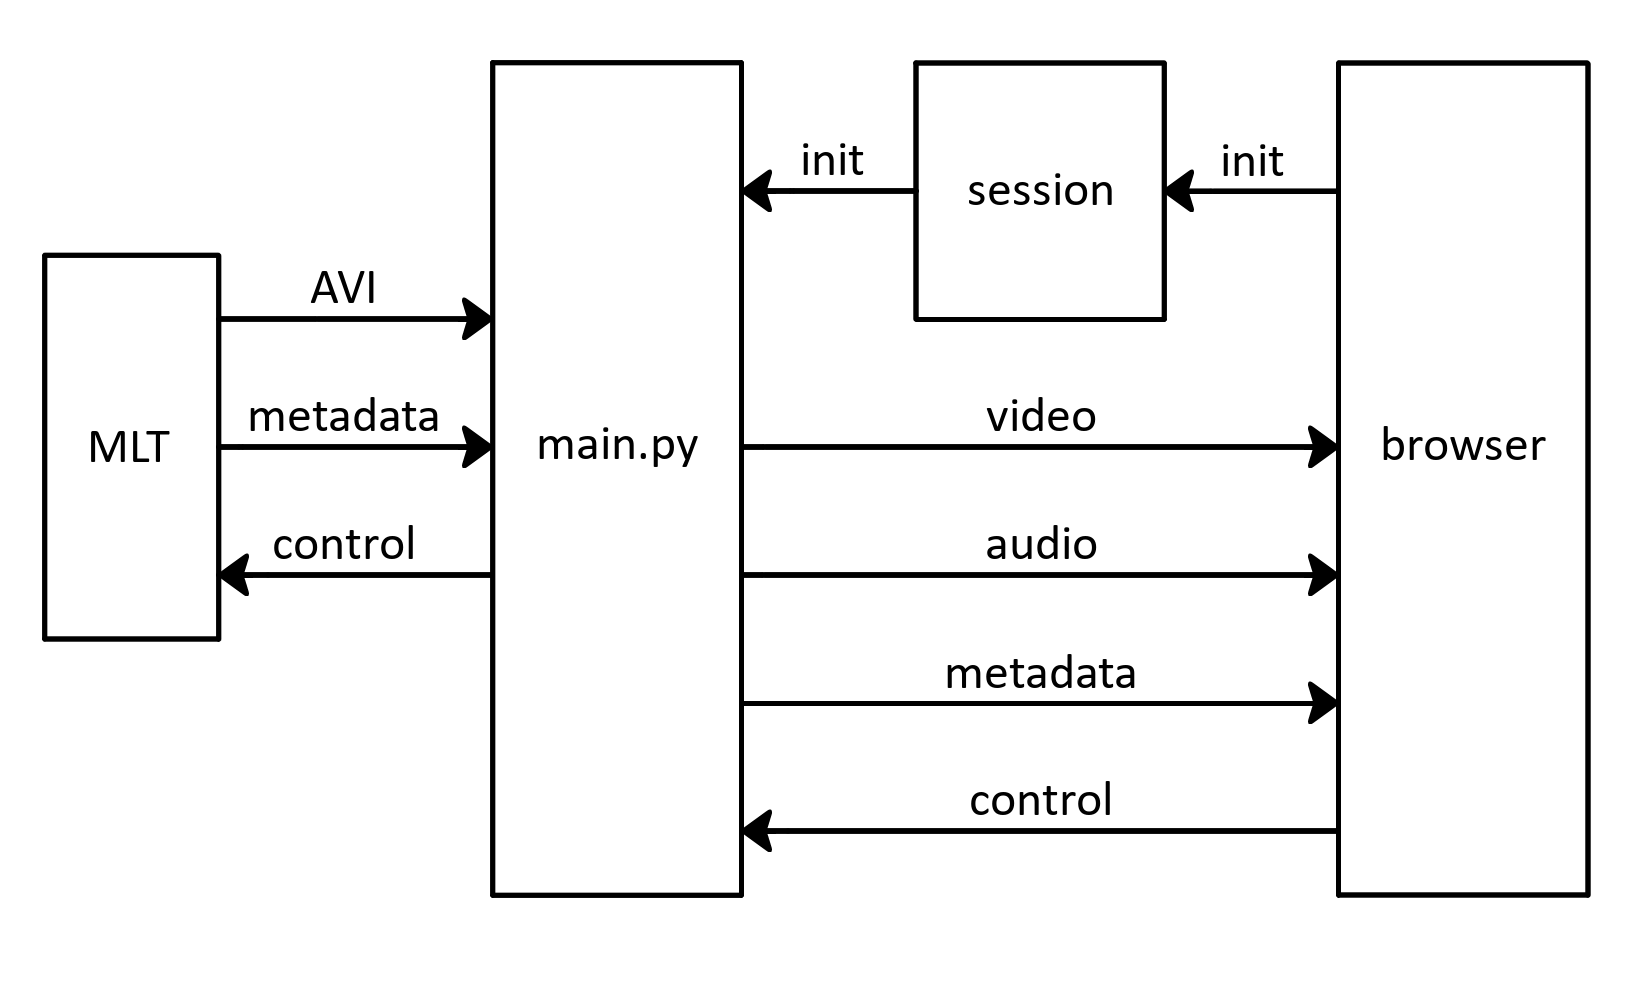
\includegraphics[width=0.8\textwidth]{IM3.png}
	\caption[System architecture]{Architecture of the system that consists out of four parts.}
	\label{figure:SA}
\end{figure}


For development and quick testing without the session service, the backend can be started in a Docker container. This has been done for the implementation for this project.







%-------------------------------------------------------------------------------------------------------
\subsection{Accurate Video} \label{subsection:accuratevideo}
% Describe the frontend

The following description of the system is based on the code base and the information from the \texttt{README} file.~\cite{RM_Frontend}

The frontend uses Node.js as its runtime environment with yarn to manage project dependencies and packages. It is developed using HyperText Markup Language (HTML), Cascading Style Sheets (CSS), and JavaScript (JS) to create the user interface.


\begin{figure}[H]
	\centering
	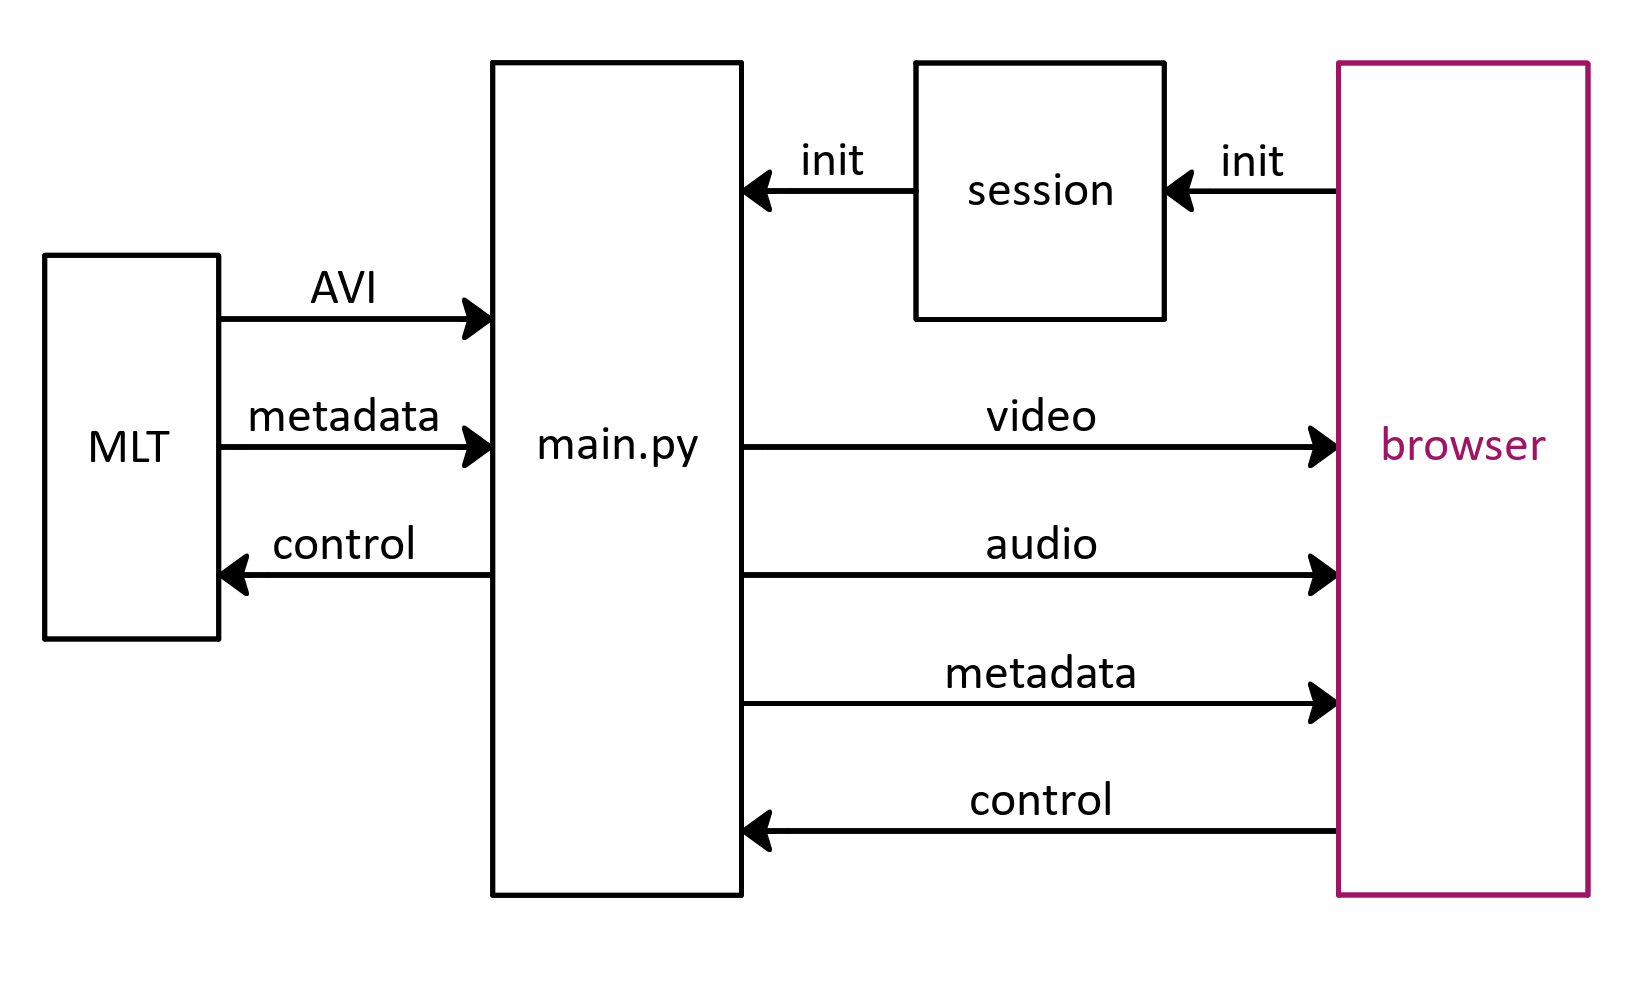
\includegraphics[width=0.5\textwidth]{IM_FE.png}
	\caption{Accurate Video in the system architecture}
	\label{figure:AS_frontend}
\end{figure}


\hypersetup{urlcolor=black}
The User Interface when playing a video in the Accurate Player at \url{http://localhost:5000/controls/jit/index.html} can be seen in Figure~\ref{figure:AV_before}. 
First, a yellow field can be seen. After clicking this, a loading screen is show and then the video can be started with clicking in the play button.


\begin{figure}[H]
	\begin{center}
		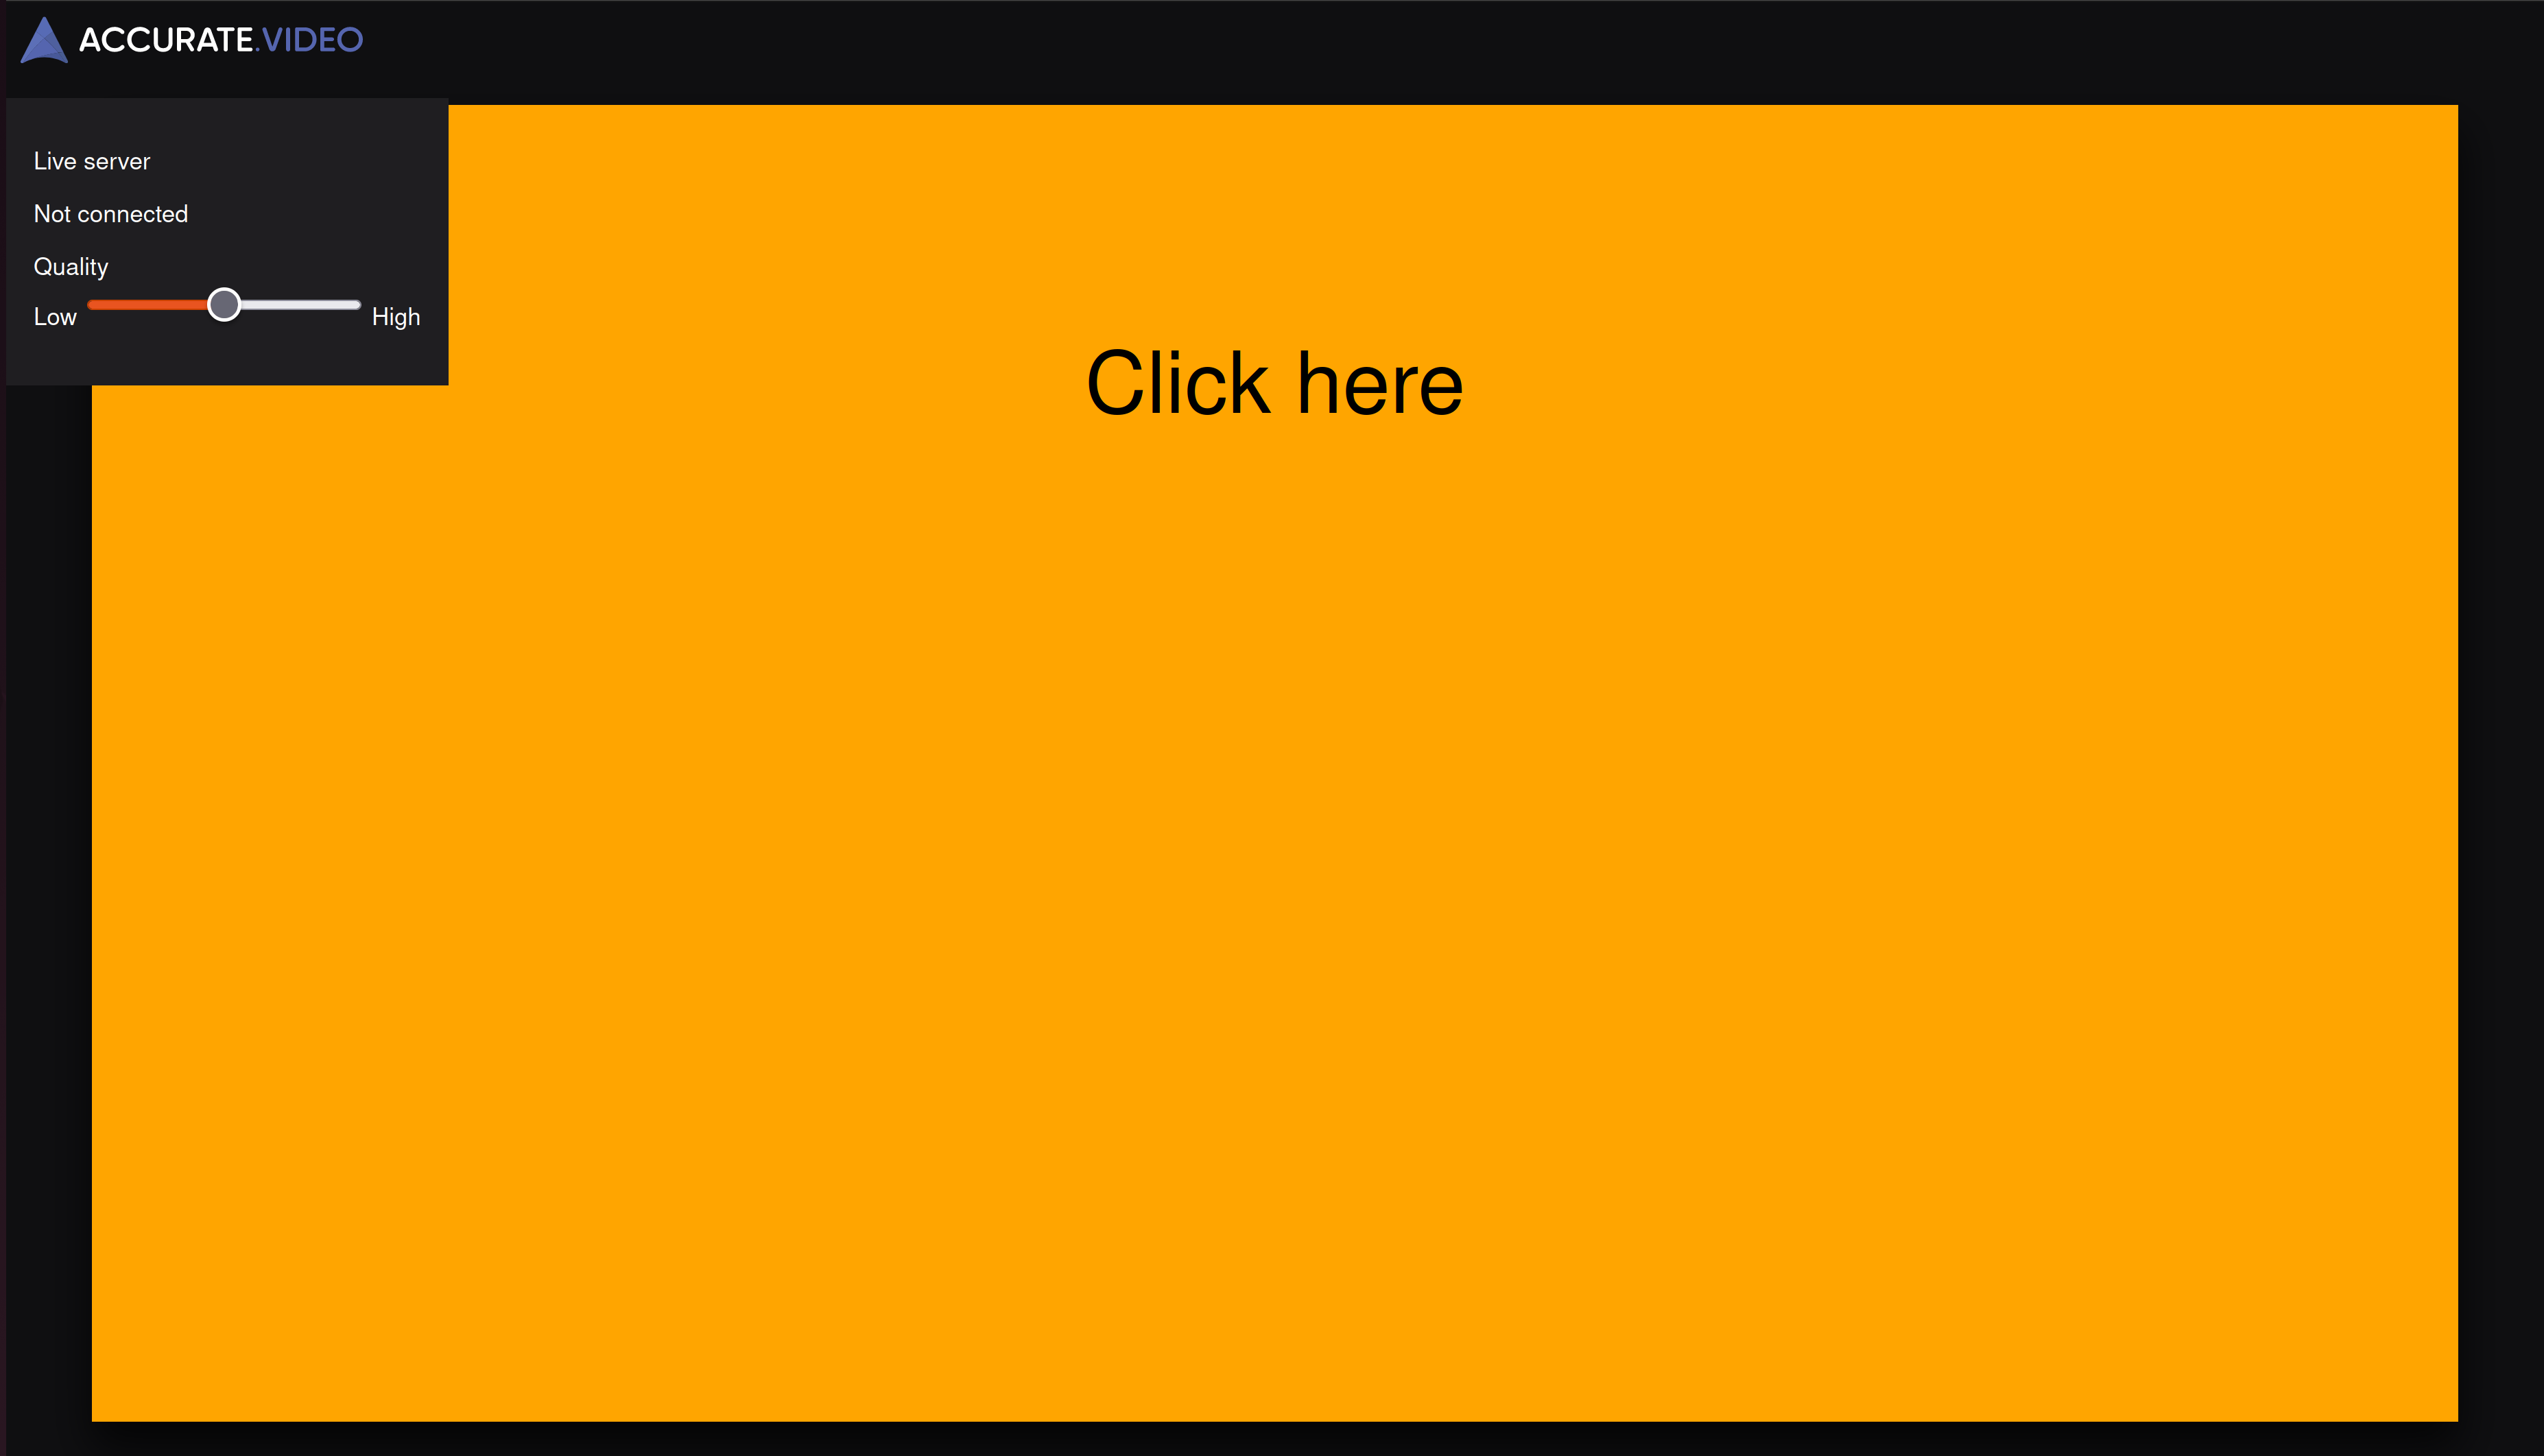
\includegraphics[width=0.32\textwidth]{AV1_before.png} \ 
		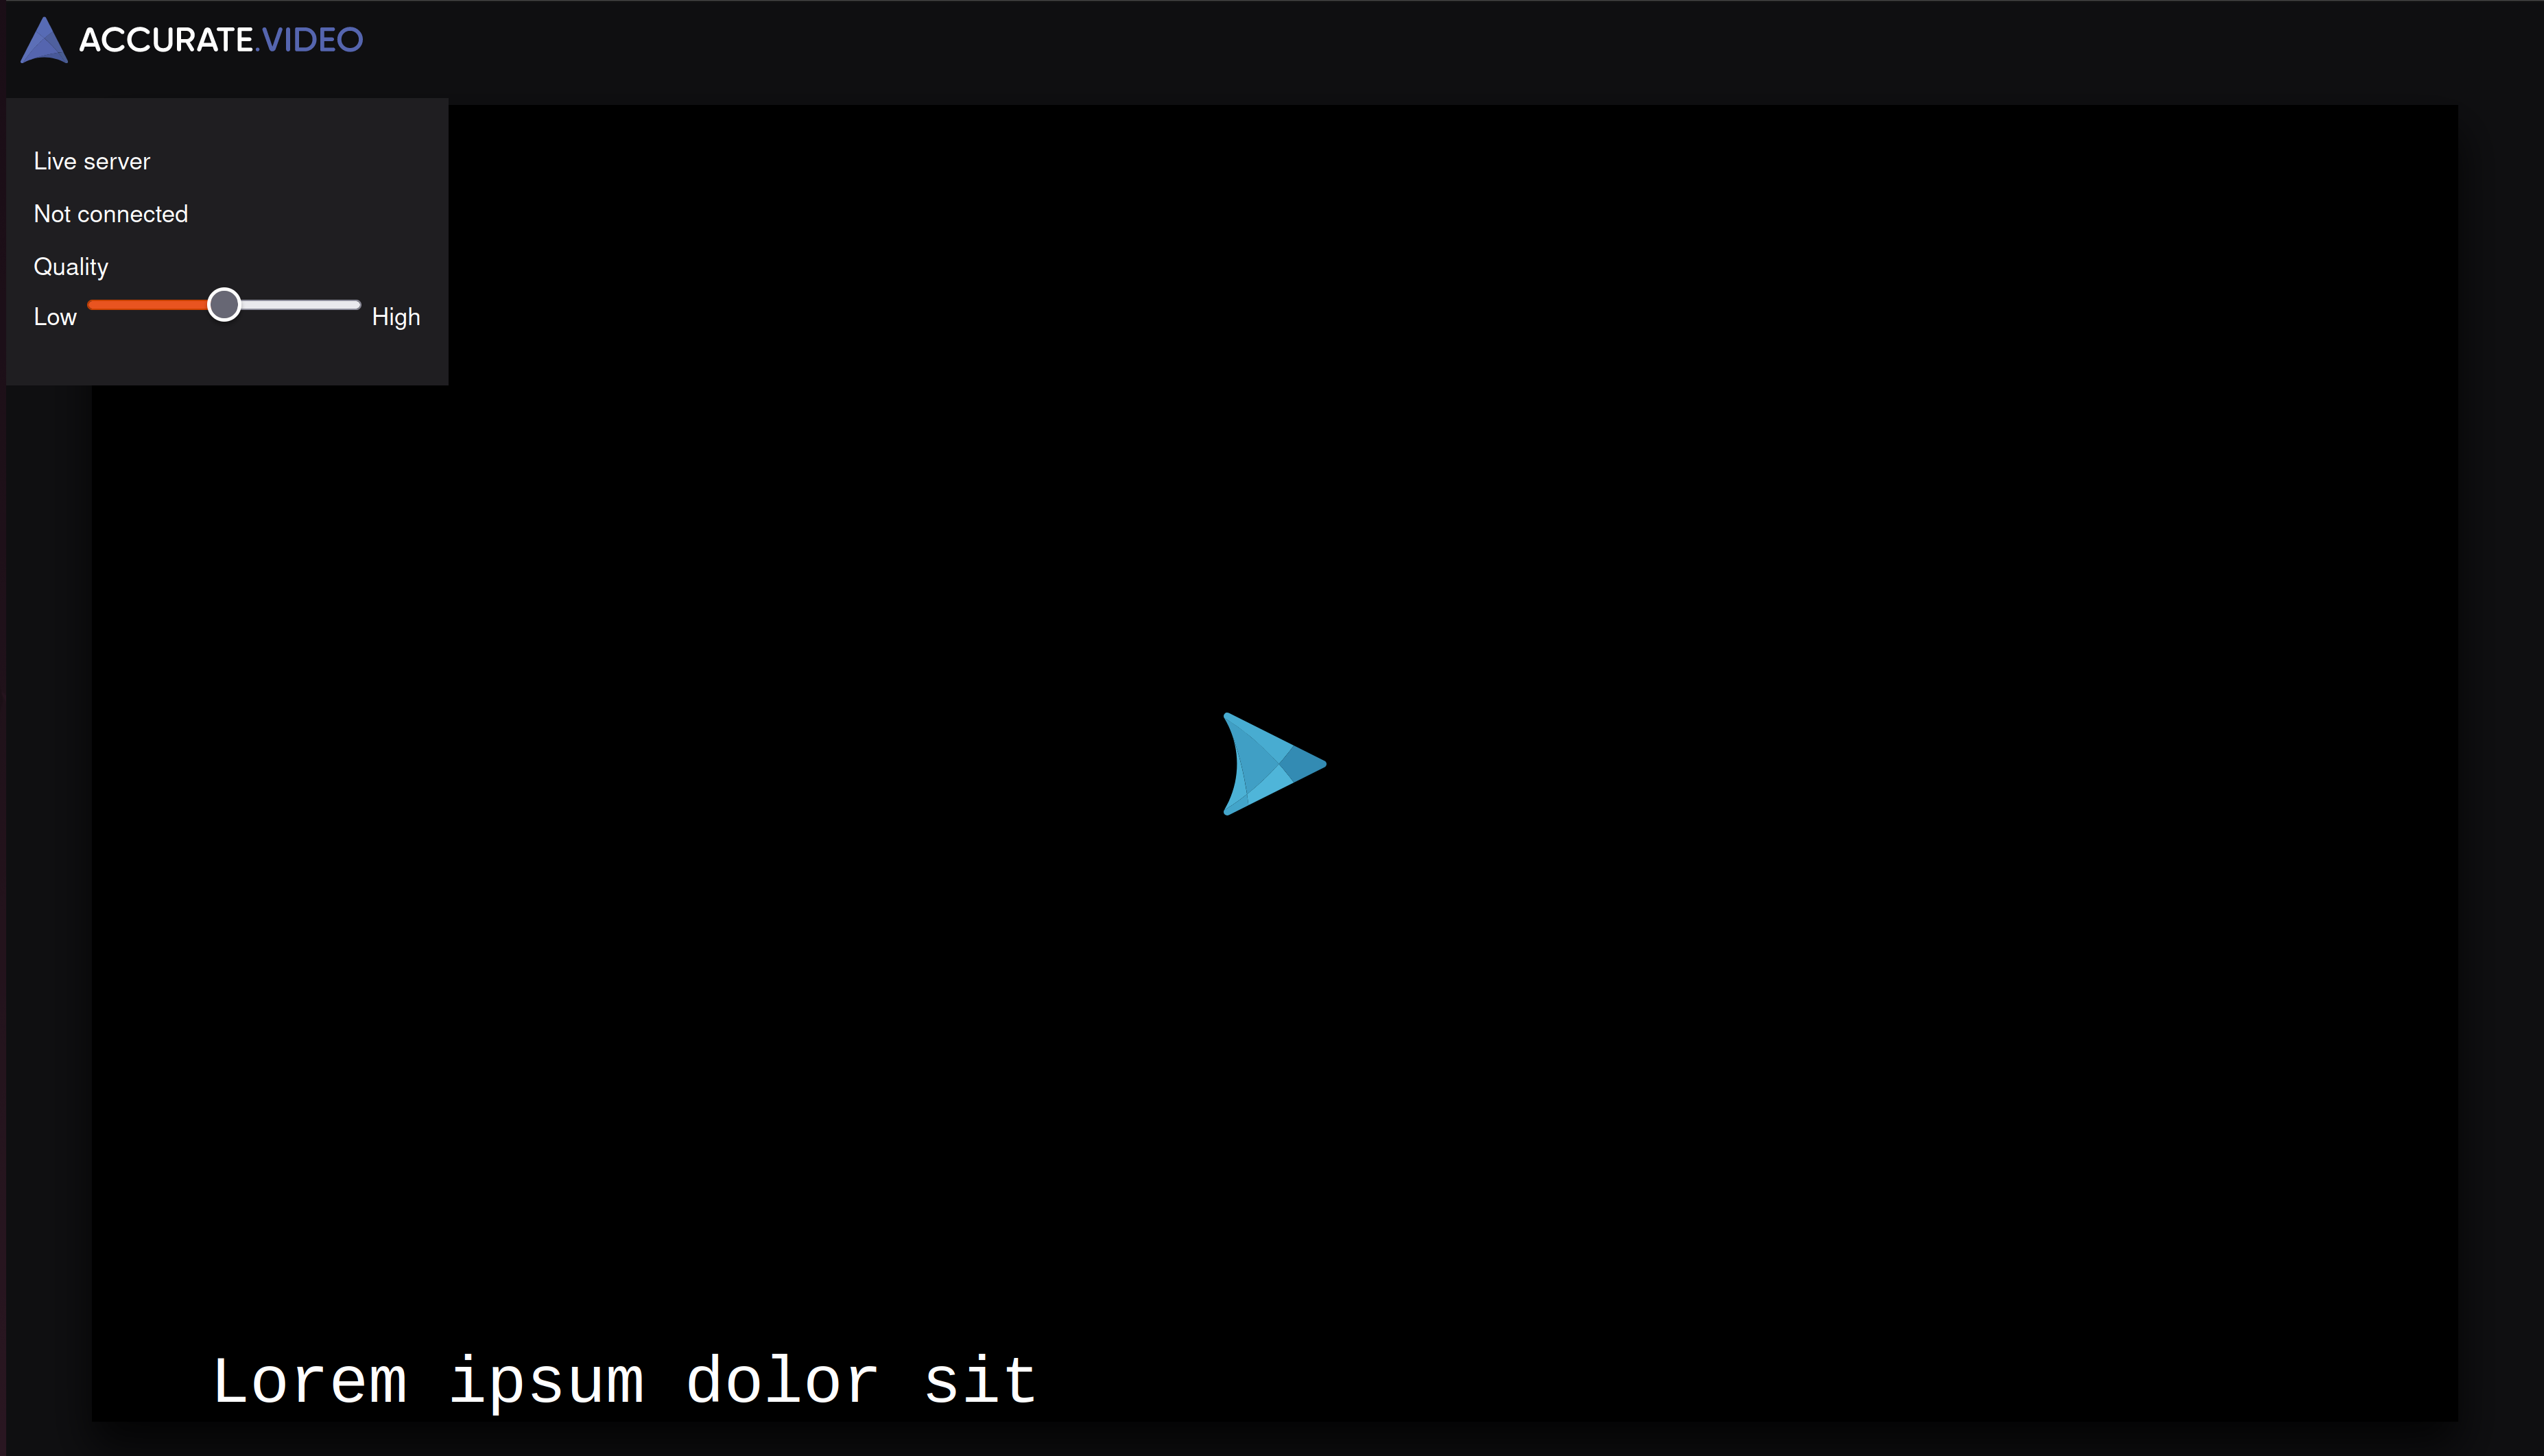
\includegraphics[width=0.32\textwidth]{AV2_before.png} \ 
		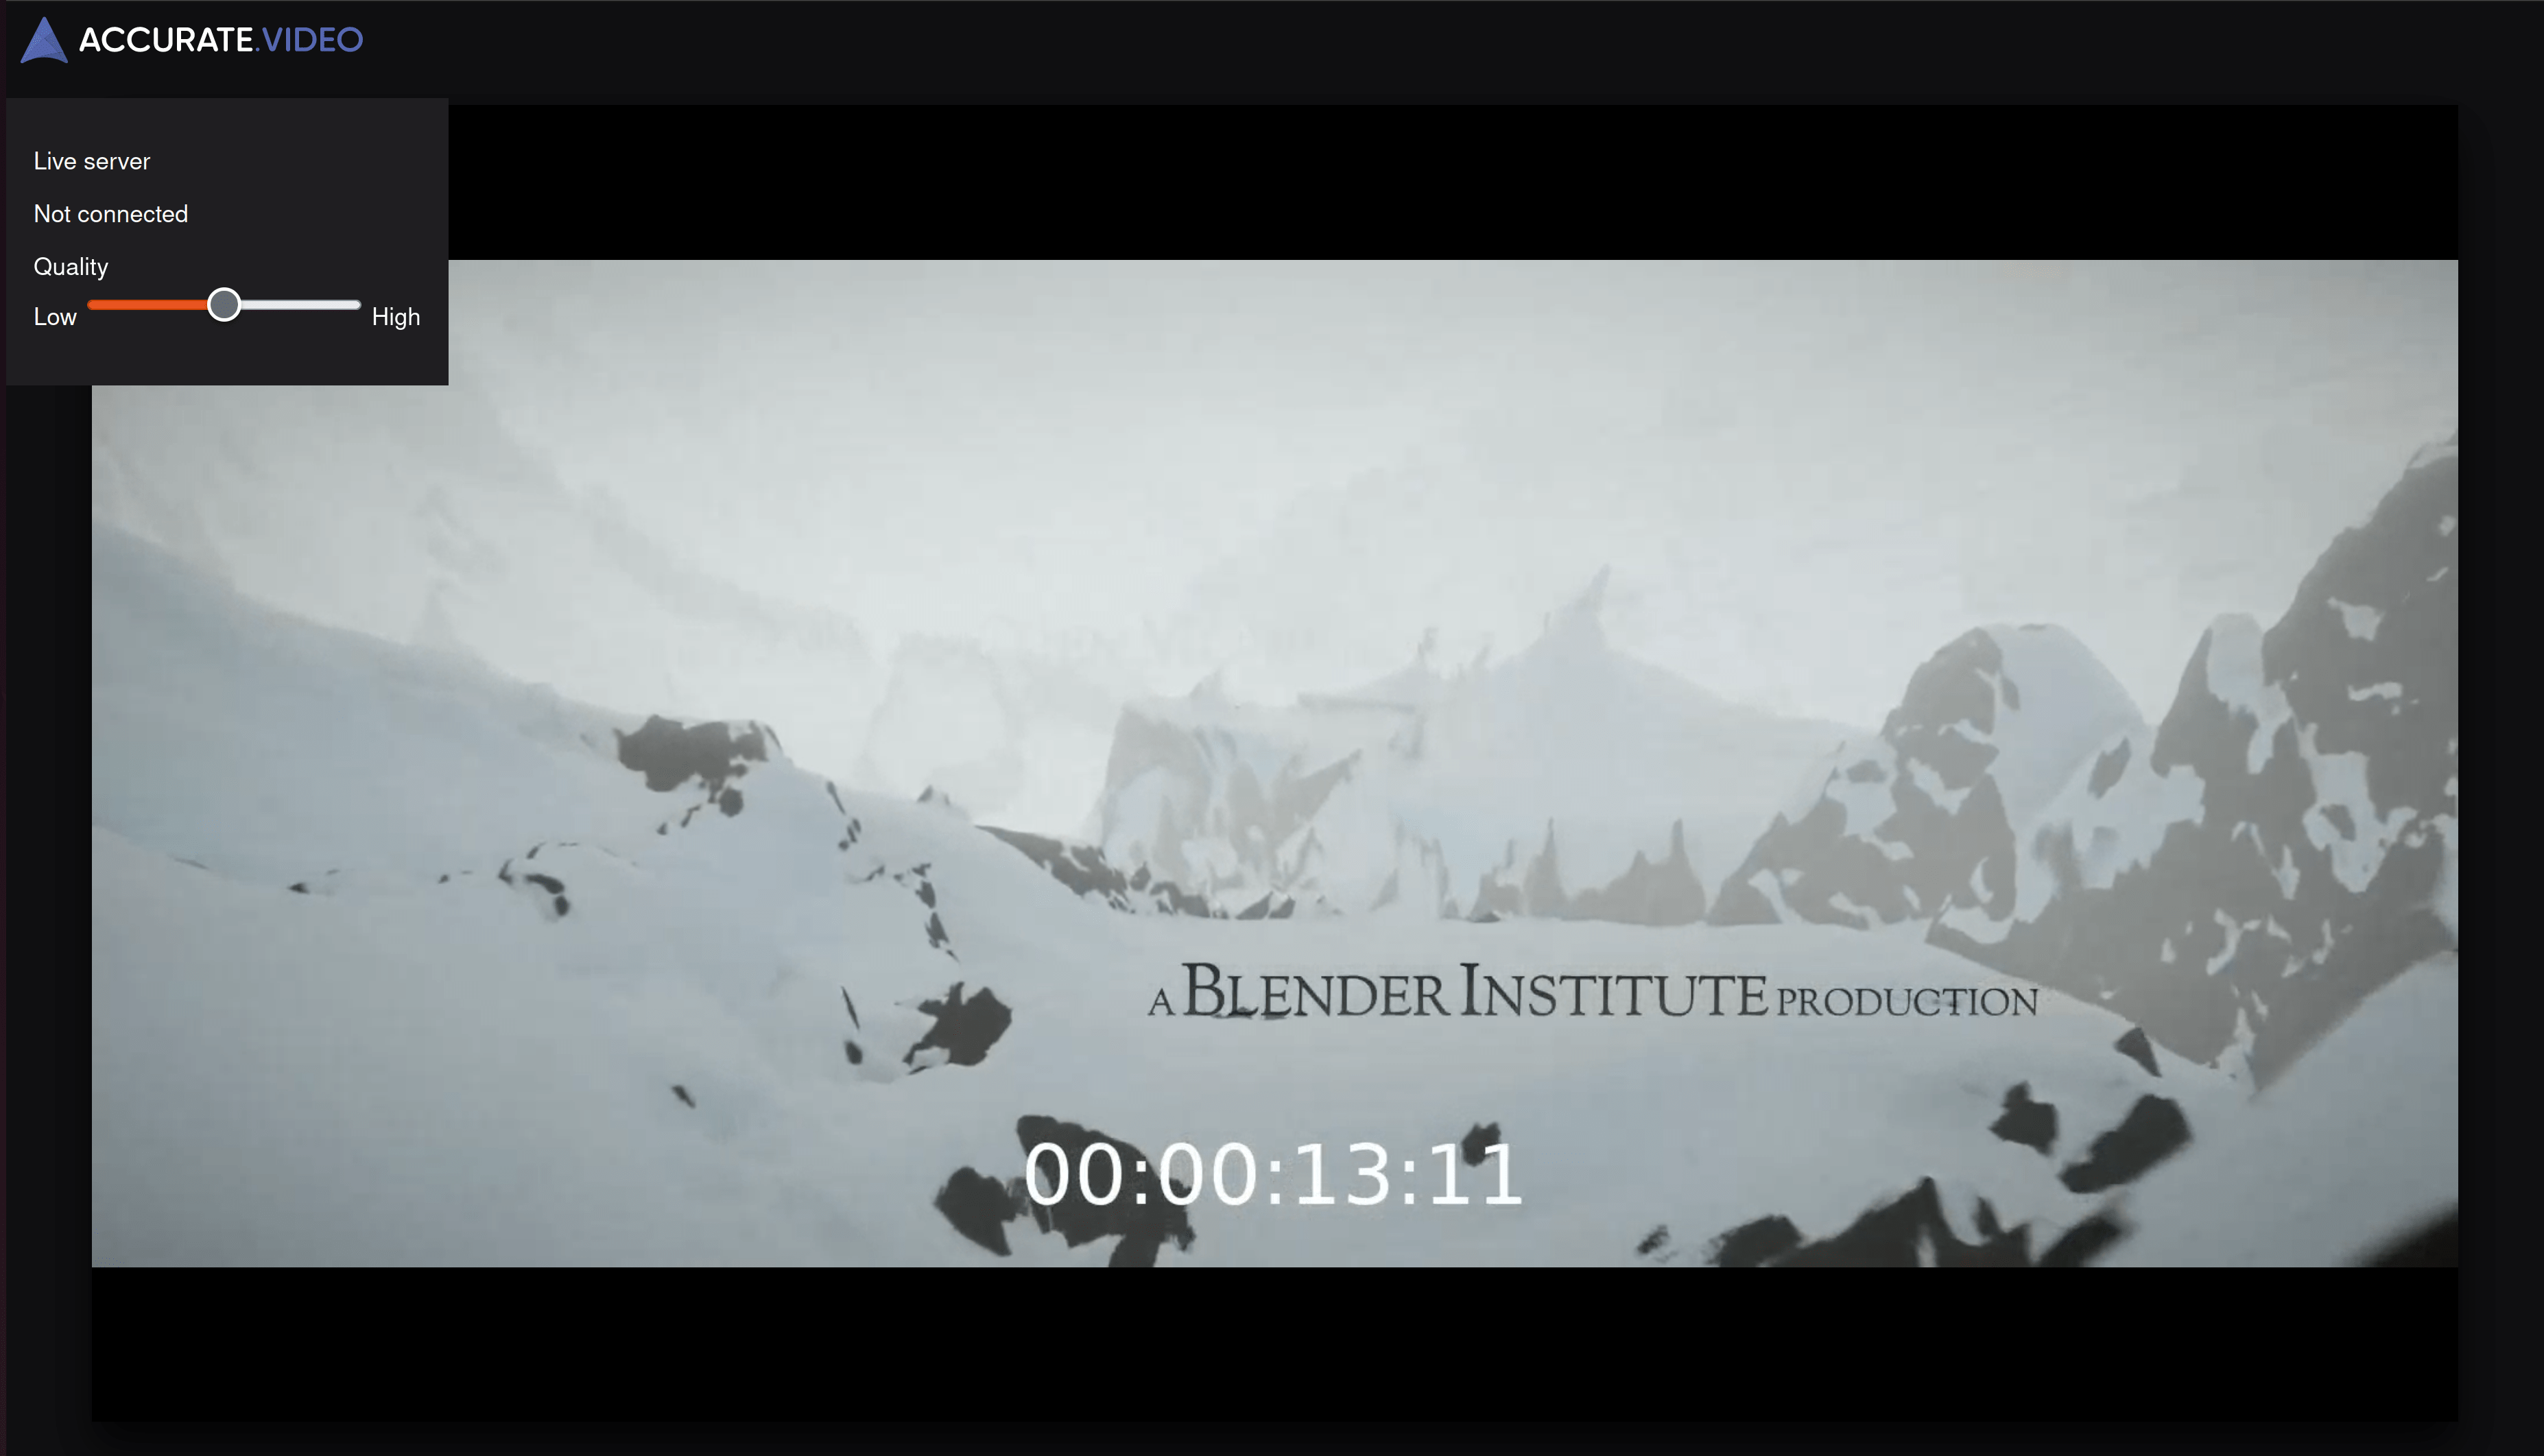
\includegraphics[width=0.32\textwidth]{AV3_before.png}
		%\cutpic{0.0cm}{0.3\textwidth}{AV2_before.png}
		%\cutpic{0.0cm}{0.3\textwidth}{AV3_before.png}
		\caption[Screenshots of the frontend.]{Screenshots of the Accurate Player when playing a video.}
		\label{figure:AV_before}
	\end{center}
\end{figure}


In addition to this, multiple control fields can be seen. Permanently fixed in the top left corner is a windows, that contains a slider to adjust the quality of the video in real time. In this project, the sliders for the RGB colour grading will be added there. This is described in Section~\ref{subsection:implementation}.
On the top left corner, two icons to expand further menus can be found. This includes one menu for muting the audio and disabling the subtitles and a menu with further settings, inlcuding the time format.
Those control fields are shown in Figure~\ref{figure:AV_details_before}.


\begin{figure}[H]
	\begin{center}
		\cutpic{0.3cm}{0.3\textwidth}{qualityslider.png}
		\cutpic{0.3cm}{0.3\textwidth}{AV_settings.png}
		\cutpic{0.3cm}{0.3\textwidth}{AV_settings2.png}
		\caption[Screenshots of the frontend.]{Screenshots of the frontend.}
		\label{figure:AV_details_before}
	\end{center}
\end{figure}







%-------------------------------------------------------------------------------------------------------
\subsection{JIT-WebRTC} \label{subsection:jit-webrtc}
% Describe the backend

The following description of the system is based on the code base and the information from the \texttt{README} file.~\cite{RM_Backend}
JIT-WebRTC is a live transcoder with a WebRTC output. As described in Section~\ref{subsection_OverviewVideoStreamingComponents}, transcoding is the conversion of one digital data format into another.~\cite{transcoding}



The backend consists of three components: Melt, \texttt{main.py} and a session service.
The system's frontend was described in Section~\ref{subsection:accuratevideo}.
In the following, the data flow between the system's components is described.

The user initiates a session through the browser, which then initiates the \texttt{main.py} script.
Control commands are then sent from the browser to \texttt{main.py} with a WebRTC data channel.
From the \texttt{main.py}, the control commands get sent to Melt via \texttt{stdout} (standard output) and \texttt{stdin} (standard input). These are the default input and output channels, that allow the Python script communication with other components.
Data written to \texttt{stdout} by the Python code can be captured or redirected and data from an external source can be read from \texttt{stdin} by the Python script.~\cite{python} The control commands are highlighted in Figure~\ref{figure:controlcommands}.

\begin{figure}[H]
	\centering
	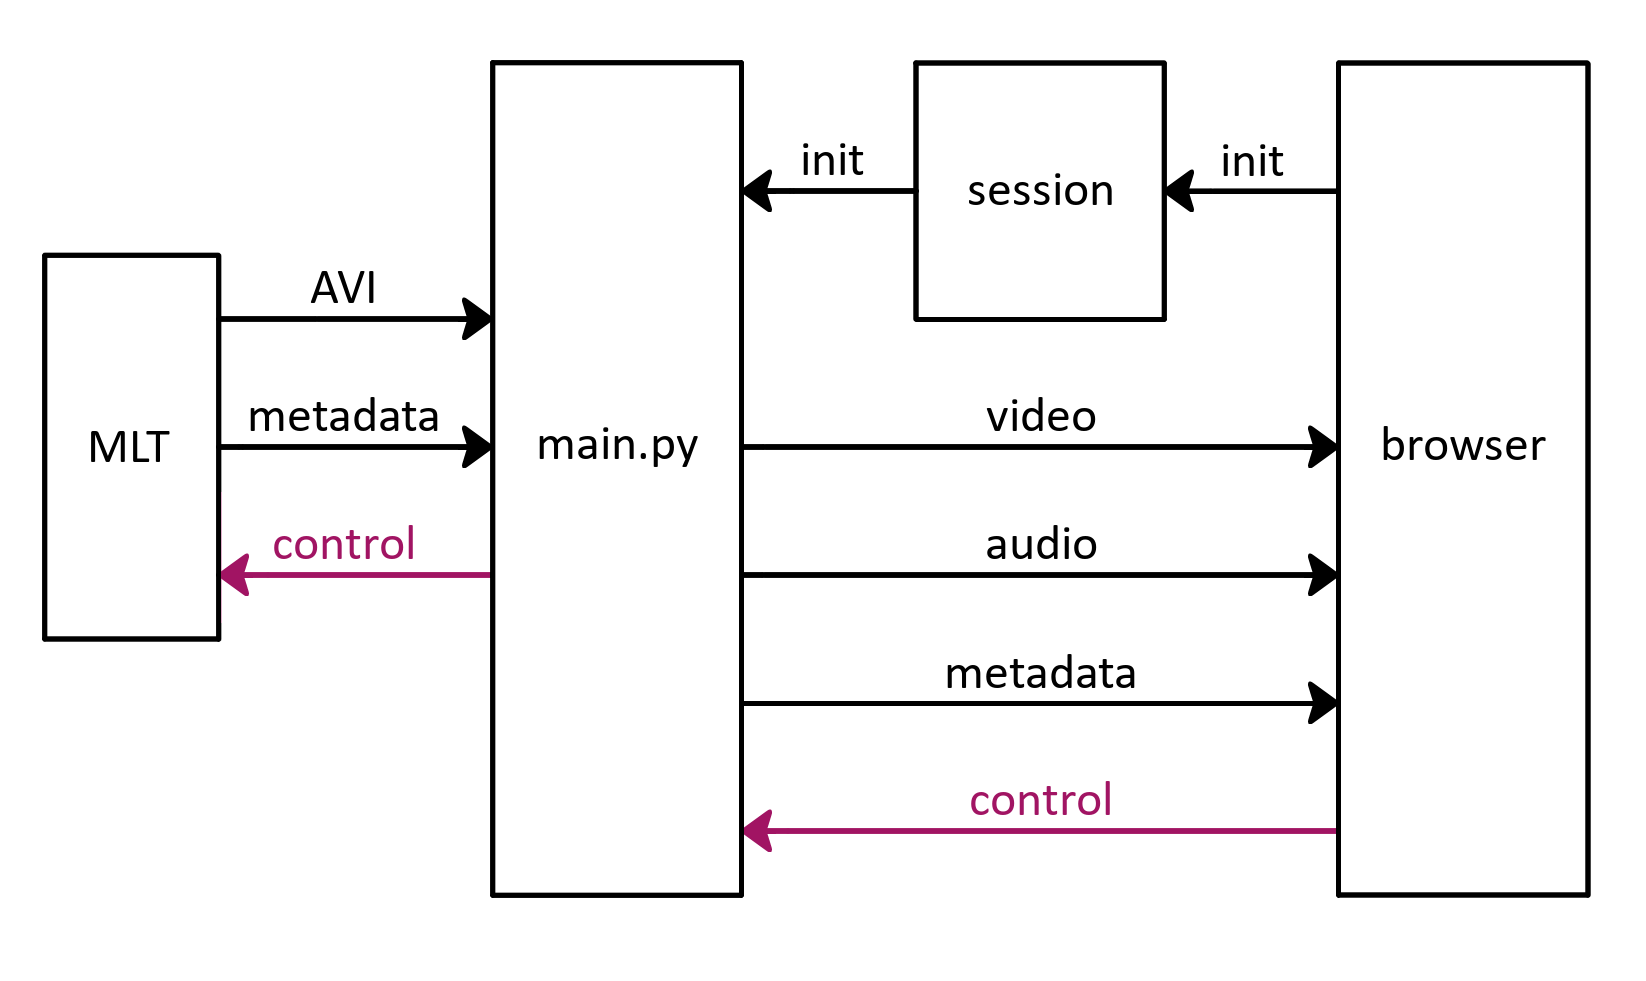
\includegraphics[width=0.5\textwidth]{IM_control.png}
	\caption{Control commands in the system architecture}
	\label{figure:controlcommands}
\end{figure}


The Melt framework then sends an AVI stream with the rendered video and audio, status messages and metadata to the \texttt{main.py}. This is highlighted in Section~\ref{figure:avimetadata}.
AVI is a file format that can contain audio and video information to allow synchronized playback of audio and video components, as described in Section~\ref{subsection_OverviewVideoStreamingComponents}.~\cite{avi} 

\begin{figure}[H]
	\centering
	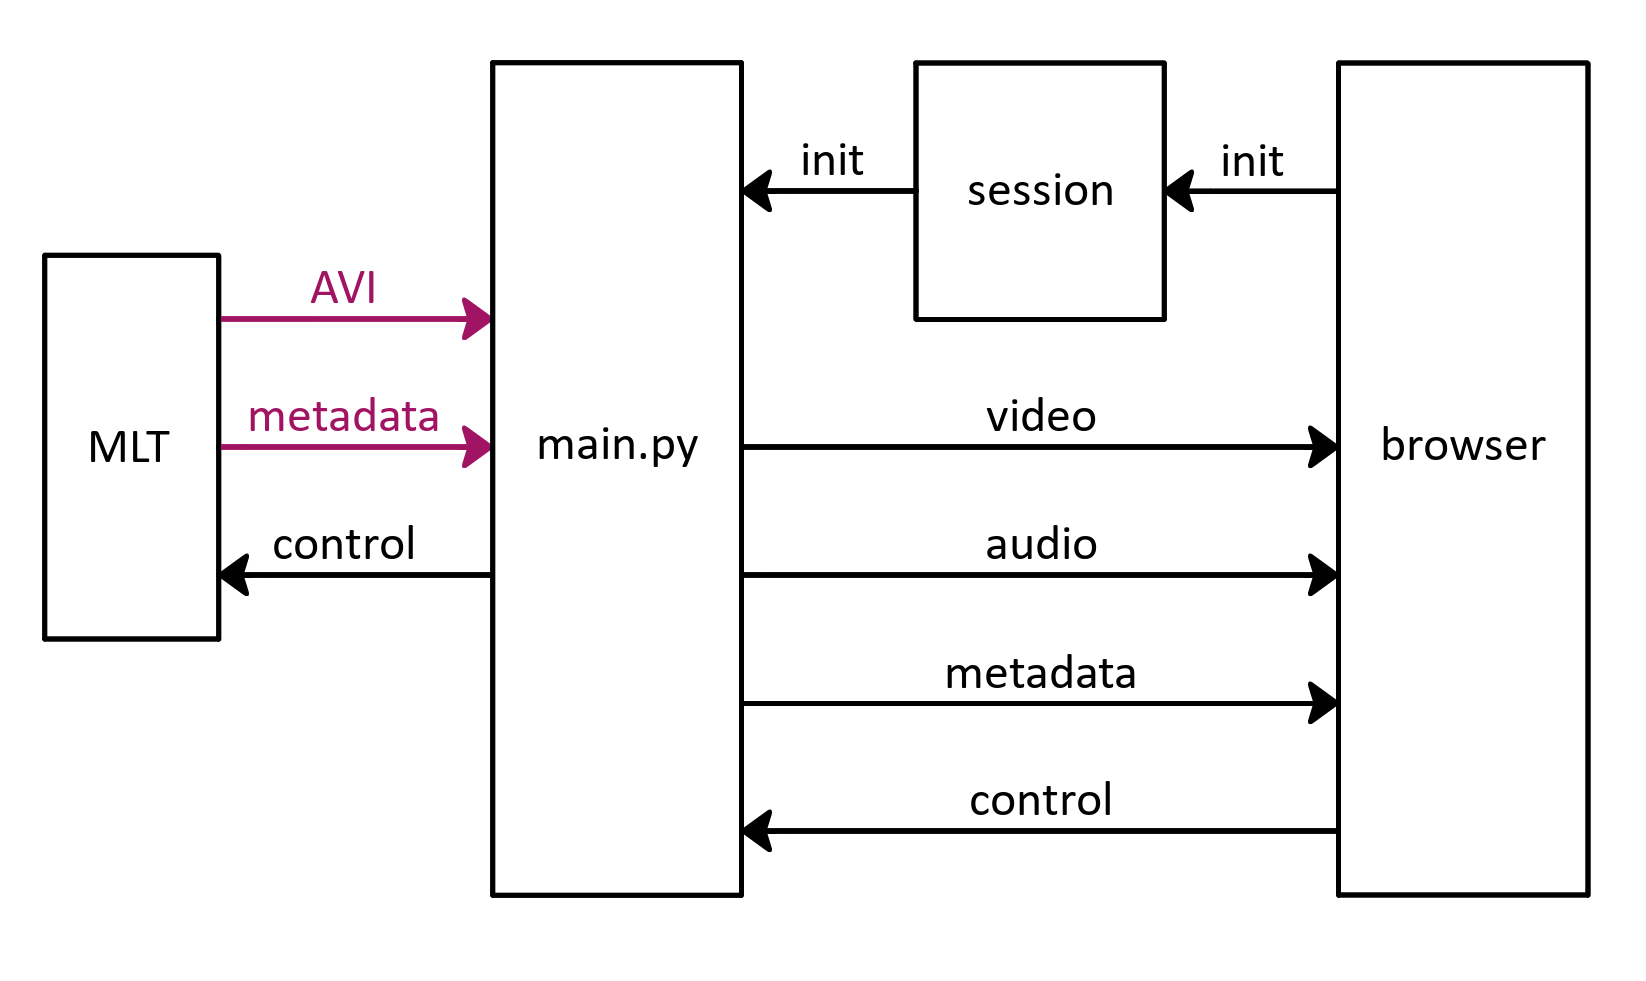
\includegraphics[width=0.5\textwidth]{IM_avi.png}
	\caption{AVI stream in the system architecture}
	\label{figure:avimetadata}
\end{figure}


Then, the audio and video from the incoming AVI stream is extracted by the \texttt{main.py} script to then encode it for sending it to the browser with WebRTC. The WebRTC connection serves as a direct communication channel between the browser and the backend, enabling real-time data exchange, involving audio, video, or other data streams. 


%It has the ability to extract specific channels from the rendered audio, to %be rendered to an stereo stream for WebRTC.
%It does not appear to be possible to encode surround sound for WebRTC, despite WebRTC using the Opus codec which is surround capable.
%This may be a limitation in `aiortc`, in WebRTC or in the browser, or all three.
%


The JavaScript client of the browser receives the video and audio to play it in the Accurate Player, which was described in Section~\ref{subsection:accuratevideo}. In addition to this, the browser
receives metadata from the \texttt{main.py} script and sends commands and responses over the control channel. This connection can be seen in Figure~\ref{figure:videoaudio}.


\begin{figure}[H]
	\centering
	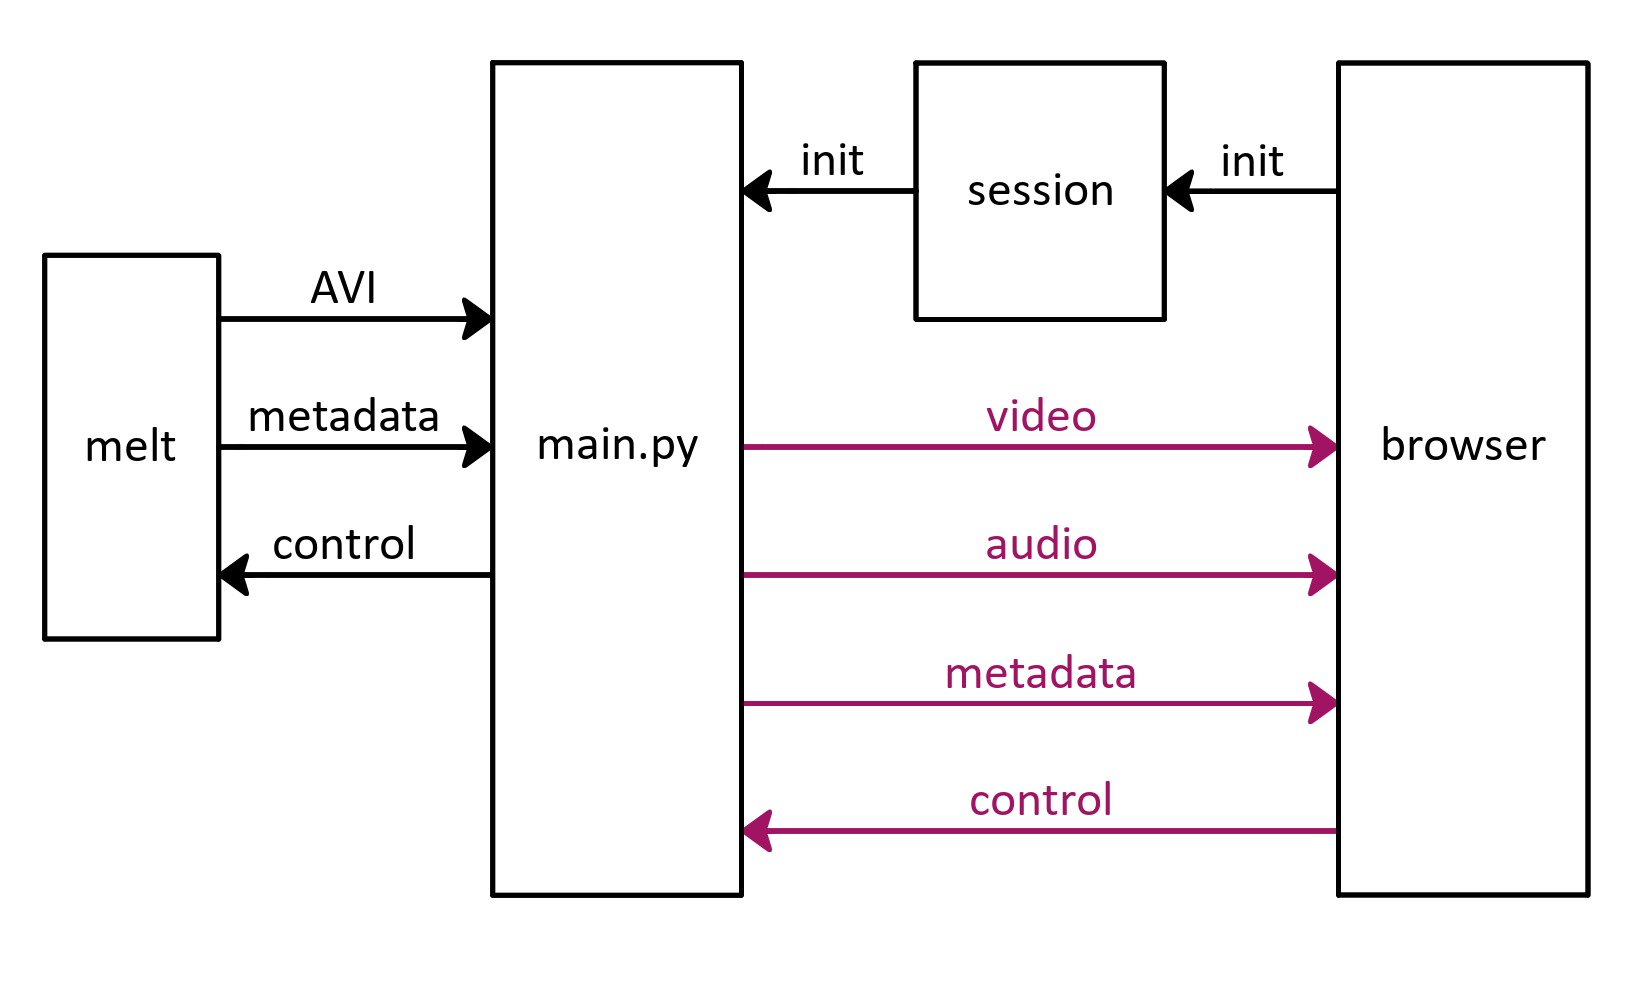
\includegraphics[width=0.5\textwidth]{IM_wrtc_control.png}
	\caption[WebRTC and control in the system architecture]{WebRTC connection and control commands in the system architecture}
	\label{figure:videoaudio}
\end{figure}

The Melt framework and the \texttt{main.py} script are started once for each JIT session.
The java-based \texttt{Session} service is designed to support the machine-to-machine interaction between the browser and the backend (\texttt{main.py} and Melt). 
The \texttt{Session} service exposes a REST API (described in Section~\ref{subsection_OverviewVideoStreamingComponents}) for initiating a JIT session. 
%
% Additionally, it leverages AWS, specifically utilizing the Auto Scaling Group (ASG) feature to manage a cluster of instances dynamically, ensuring scalability and efficient distribution of JIT sessions across the instances in the cluster.
%
% AWS
%2. **AWS (Amazon Web Services):**
%- **Definition:** AWS is a cloud computing platform provided by Amazon. It offers a wide range of services, including computing power, storage, databases, machine learning, and more, allowing businesses to scale and grow without the need for significant upfront investments in physical infrastructure.
%
% ASG cluster
%3. **ASG Cluster (Auto Scaling Group):**
%- **Definition:** An Auto Scaling Group is an AWS service that automatically adjusts the number of compute instances (e.g., virtual machines) in response to changes in demand or other specified conditions. It helps ensure that the desired number of instances are available to handle varying workloads.
%
%
%
%`session` is a Java-based service that presents a REST api that can be used to start a new JIT session given a description of the media to use. It also has support for managing a full ASG cluster on AWS, and distribute new JIT sessions on the instances in 
%the ASG.
%
%For more information on each component see:
%* [`melt`](https://github.com/sirf/mlt.git)
%* [`main.py`](jit/README.md)
%* [`session`](session/README.md)
%

For development and quick testing without the session service, JIT can be started in a Docker container. This has been done for the implementation for this project.


%\begin{figure}[H]
%	\centering
%	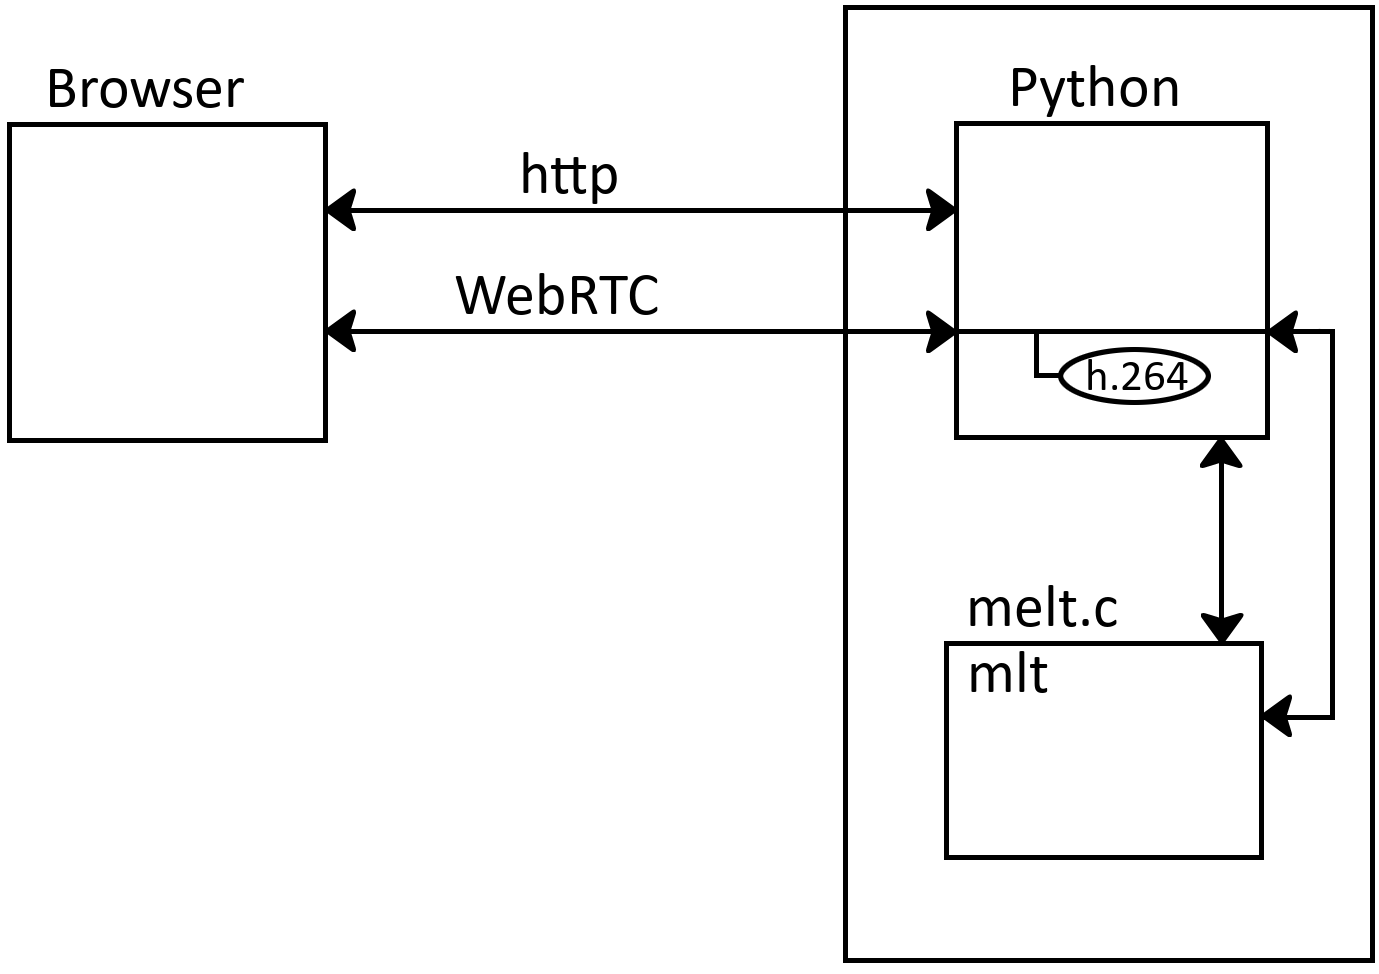
\includegraphics[width=0.6\textwidth]{IM2.png}
%	\caption{System architecture when run in a docker container.}
%\end{figure}


%## Development
%
%For development and quick testing without the session service, on can either start JIT as a docker, or run JIT directly on your computer. The latter has some problems if you're on an Apple ARM.
%
%Run the docker:
%
%`docker/main/main.sh --threads 16 --port 8080 $VIDEOFILE`
%
%Where `$VIDEOFILE` is either a local path or a URL. `threads` and `port` are both optional, with current default values set to 72 threads and port 8080.
%
%To run JIT directly, see [`jit/README.md`](jit/README.md).
%
%### Open Docker IPs
%
%Your Docker container will get an IP in the style of 172.17.0.\*. Using e.g. Docker CE on Linux this IP will be reachable from outside the container. However, on Docker Desktop for Mac, this IP will not be opened. This will cause problems. There is a service that can fix this. You **install and activate it once** by doing this:
%
%```
%# Install via Homebrew
%brew install chipmk/tap/docker-mac-net-connect
%
%# Run the service and register it to launch at boot
%sudo brew services start chipmk/tap/docker-mac-net-connect
%```
%
%
%## Deployment
%
%Currently the only way supported for deployment is by using EC2 instances on AWS. An AMI is created by CI on release, containing a 
%local instance of the `session-service`, together with `main.py`, `melt` and anything else needed to start JIT processes on the EC2 
%instance. For more information about what the AMI contains, and how configuration can be fed to it see [`ami/README.md`](ami/README.md).
%
%### Terraform
%
%Terraform modules are supplied that simplify setup of either single EC2 instances or a full ASG cluster of instances, including 
%`session-service` running as an orchestrator on ECS. See [`terraform/README.md`](terraform/README.md) for more information on 
%available modules, their parameters and outputs.
%





% \newpage
%-------------------------------------------------------------------------------------------------------
\subsection{Melt Filter Comparison} \label{subsection:meltfilter}



The goal for this thesis project is to adjust the RGB values of a video with sliders. For this purpose, various Melt filters that seemed suitable were examined and compared to identify the most suitable ones for implementing this functionality. RGB colour representation was described in Section~\ref{subsection:RGB} and the Melt framework was described in Section~\ref{subsection:melt}.

In the following, a selection of filters, that influence the RGB representation of the video are listed. This includes the filter name, description and possible parameters from the Melt website.~\cite{melt_filters} Only the relevant parameters will be listed.
Those filters were then executed locally, to compare the visual results of applying them.
The Melt filters \texttt{avfilter.colorbalance}, \texttt{avfilter\-.colorchannelmixer} and \texttt{frei0r\-.coloradj\_RGB} are listed with their description and parameters in Table~\ref{table:filter}. Other Melt filters that change the visual appearance of the video can be seen in Appendix~\ref{appendix:differentMeltFilter}.


\begin{table}[H]
	\footnotesize
	\begin{tabular}{lp{4.4cm}p{4.5cm}}
		\toprule
		Name & Description & Parameters \\
		\midrule
		\texttt{avfilter.colorbalance} & Adjust the colour balance & 
		\tiny{
		\texttt{av.rs}: set red shadows \newline 
		\texttt{av.gs}: set green shadows \newline 
		\texttt{av.bs}: set blue shadows \newline 
		\texttt{av.rm}: set red mid tones \newline 
		\texttt{av.gm}: set green mid tones \newline 
		\texttt{av.bm}: set blue mid tones \newline 
		\texttt{av.rh}: set red highlights \newline 
		\texttt{av.gh}: set green highlights \newline 
		\texttt{av.bh}: set blue highlights}
		\\
		\texttt{avfilter.colorchannelmixer} & Adjust colours by mixing colour channels & 
		\tiny{
		\texttt{av.rr}: set red gain for red channel \newline 
		\texttt{av.rg}: set green gain for red channel \newline 
		\texttt{av.rb}: set blue gain for red channel \newline 
		\texttt{av.ra}: set alpha gain for red channel \newline 
		\texttt{av.gr}: set red gain for green channel \newline 
		\texttt{av.gg}: set green gain for green channel \newline 
		\texttt{av.gb}: set blue gain for green channel \newline 
		\texttt{av.ga}: set alpha gain for green channel \newline 
		\texttt{av.br}: set red gain for blue channel \newline 
		\texttt{av.bg}: set green gain for blue channel \newline 
		\texttt{av.bb}: set blue gain for blue channel \newline 
		\texttt{av.ba}: set red gain for alpha channel \newline 
		\texttt{av.ar}: set red gain for alpha channel \newline 
		\texttt{av.ag}: set green gain for alpha channel \newline 
		\texttt{av.ab}: set blue gain for alpha channel \newline 
		\texttt{av.aa}: set alpha gain for alpha channel}
		\\
		\texttt{frei0r.coloradj\_RGB} & Simple colour adjustment & 
		\tiny{
		\texttt{R}: amount of red \newline 
		\texttt{G}: amount of green \newline 
		\texttt{B}: amount of blue}
		\\
		\bottomrule
	\end{tabular}
	\caption[List of Melt filters that influence the colour of a video.]{List of different Melt filters that influence the colour of a video with their name, description and parameters.}
	\label{table:filter}
\end{table}



%Execution of \texttt{melt https://s3.eu-central-1.amazonaws.com/accurate-player\--demo-assets/timecode/sintel-2048-timecode-stereo.mp4 \\ -filter avfilter.colorbalance av.rs=1 av.gm=1 av.bh=1}:


%\begin{minipage}{0.5\textwidth}
%	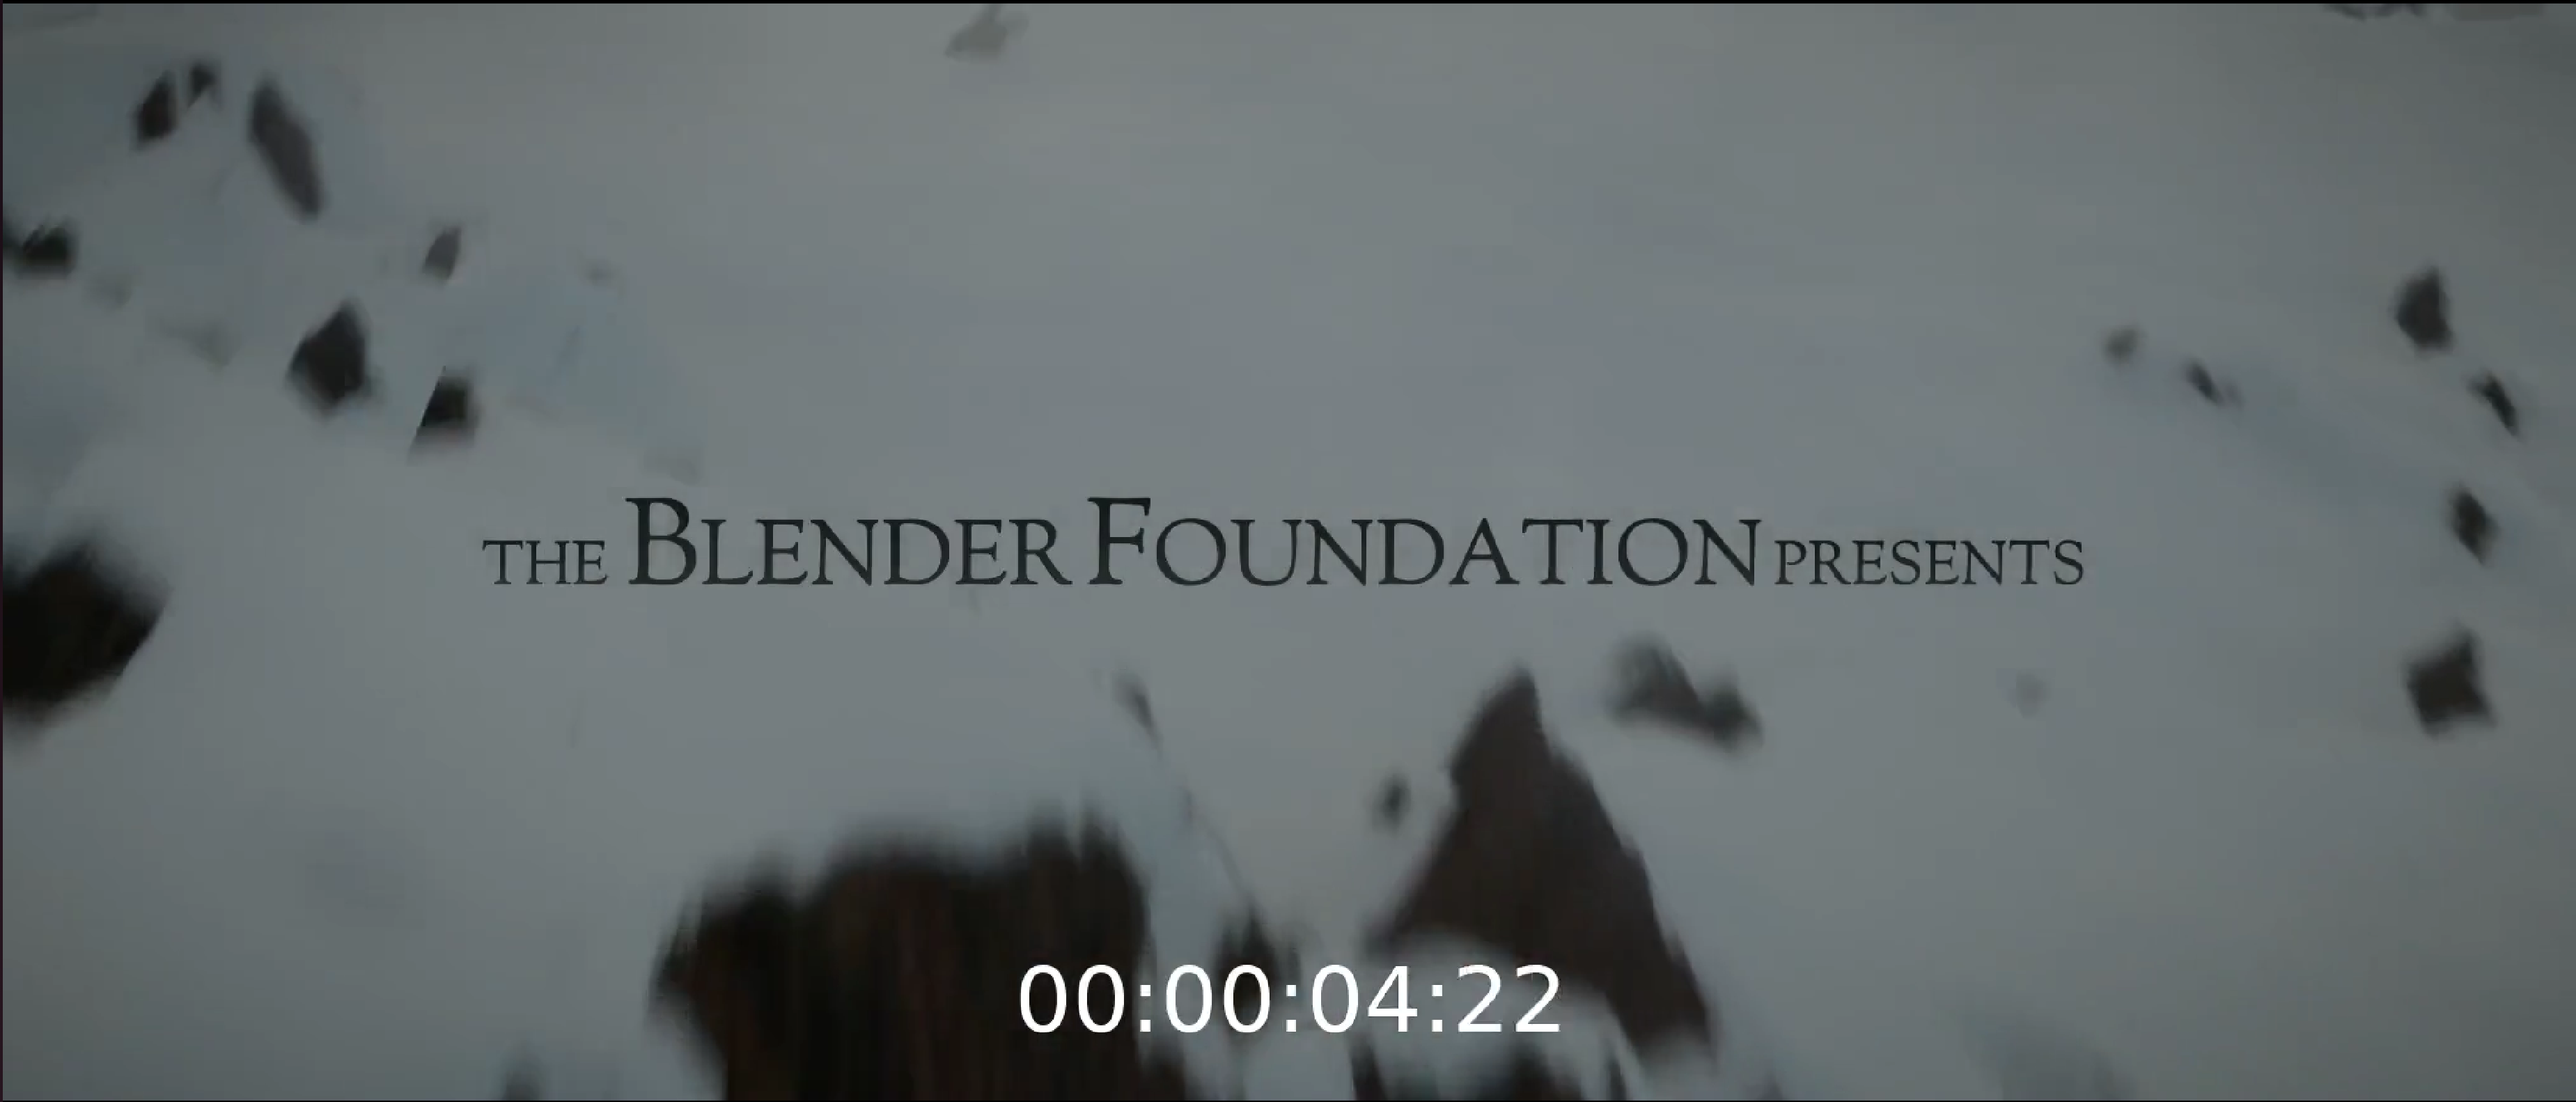
\includegraphics[width=0.9\textwidth]{colourdefault.png}
%	Original colours
%\end{minipage}\begin{minipage}{0.5\textwidth}
%	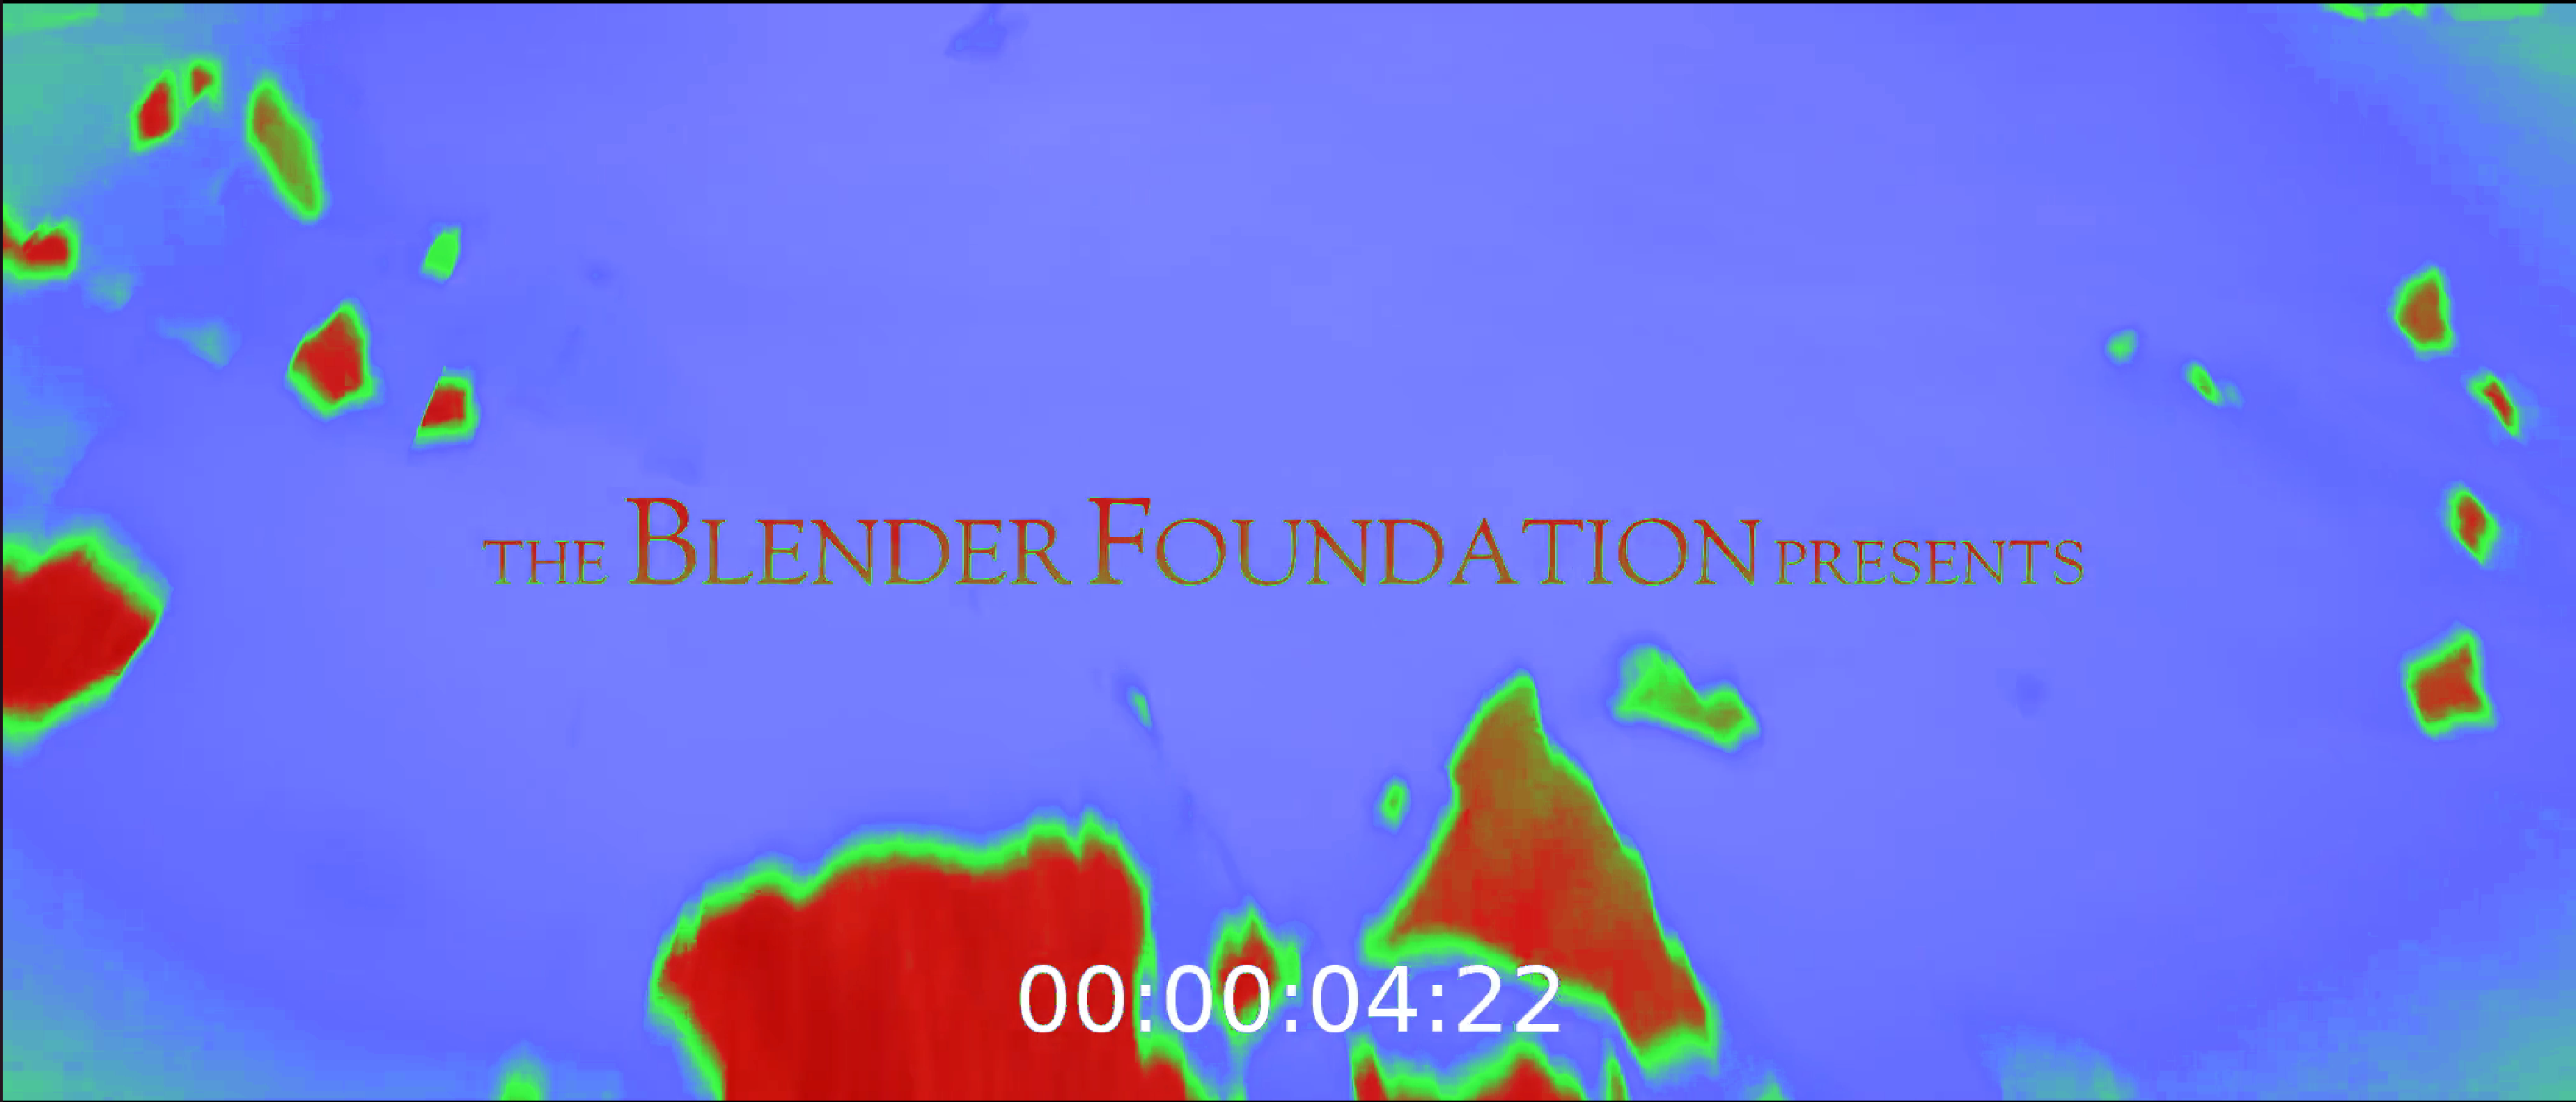
\includegraphics[width=0.9\textwidth]{colourhigh.png}
%	Colours with \texttt{av.rs=1} \texttt{av.gm=1} \texttt{av.bh=1}
%\end{minipage}

%Adding filter to \texttt{local\_melt.py} to execute it in the Accurate Player using JIT:
%`
%\begin{center}
%	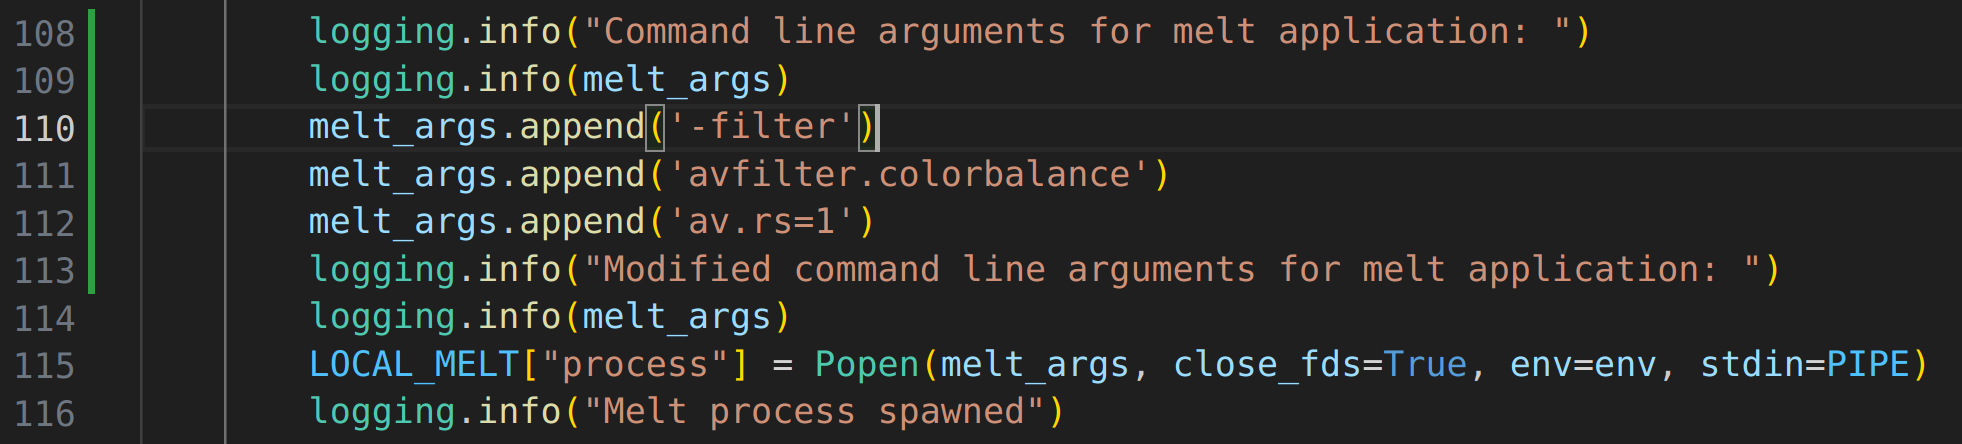
\includegraphics[height=0.13\textwidth]{code.png}
%	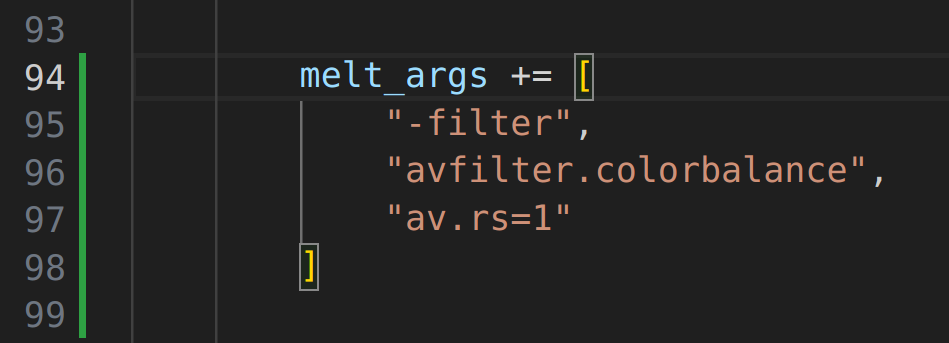
\includegraphics[height=0.13\textwidth]{codecleaner.png}
%\end{center}
%
%\begin{center}
%	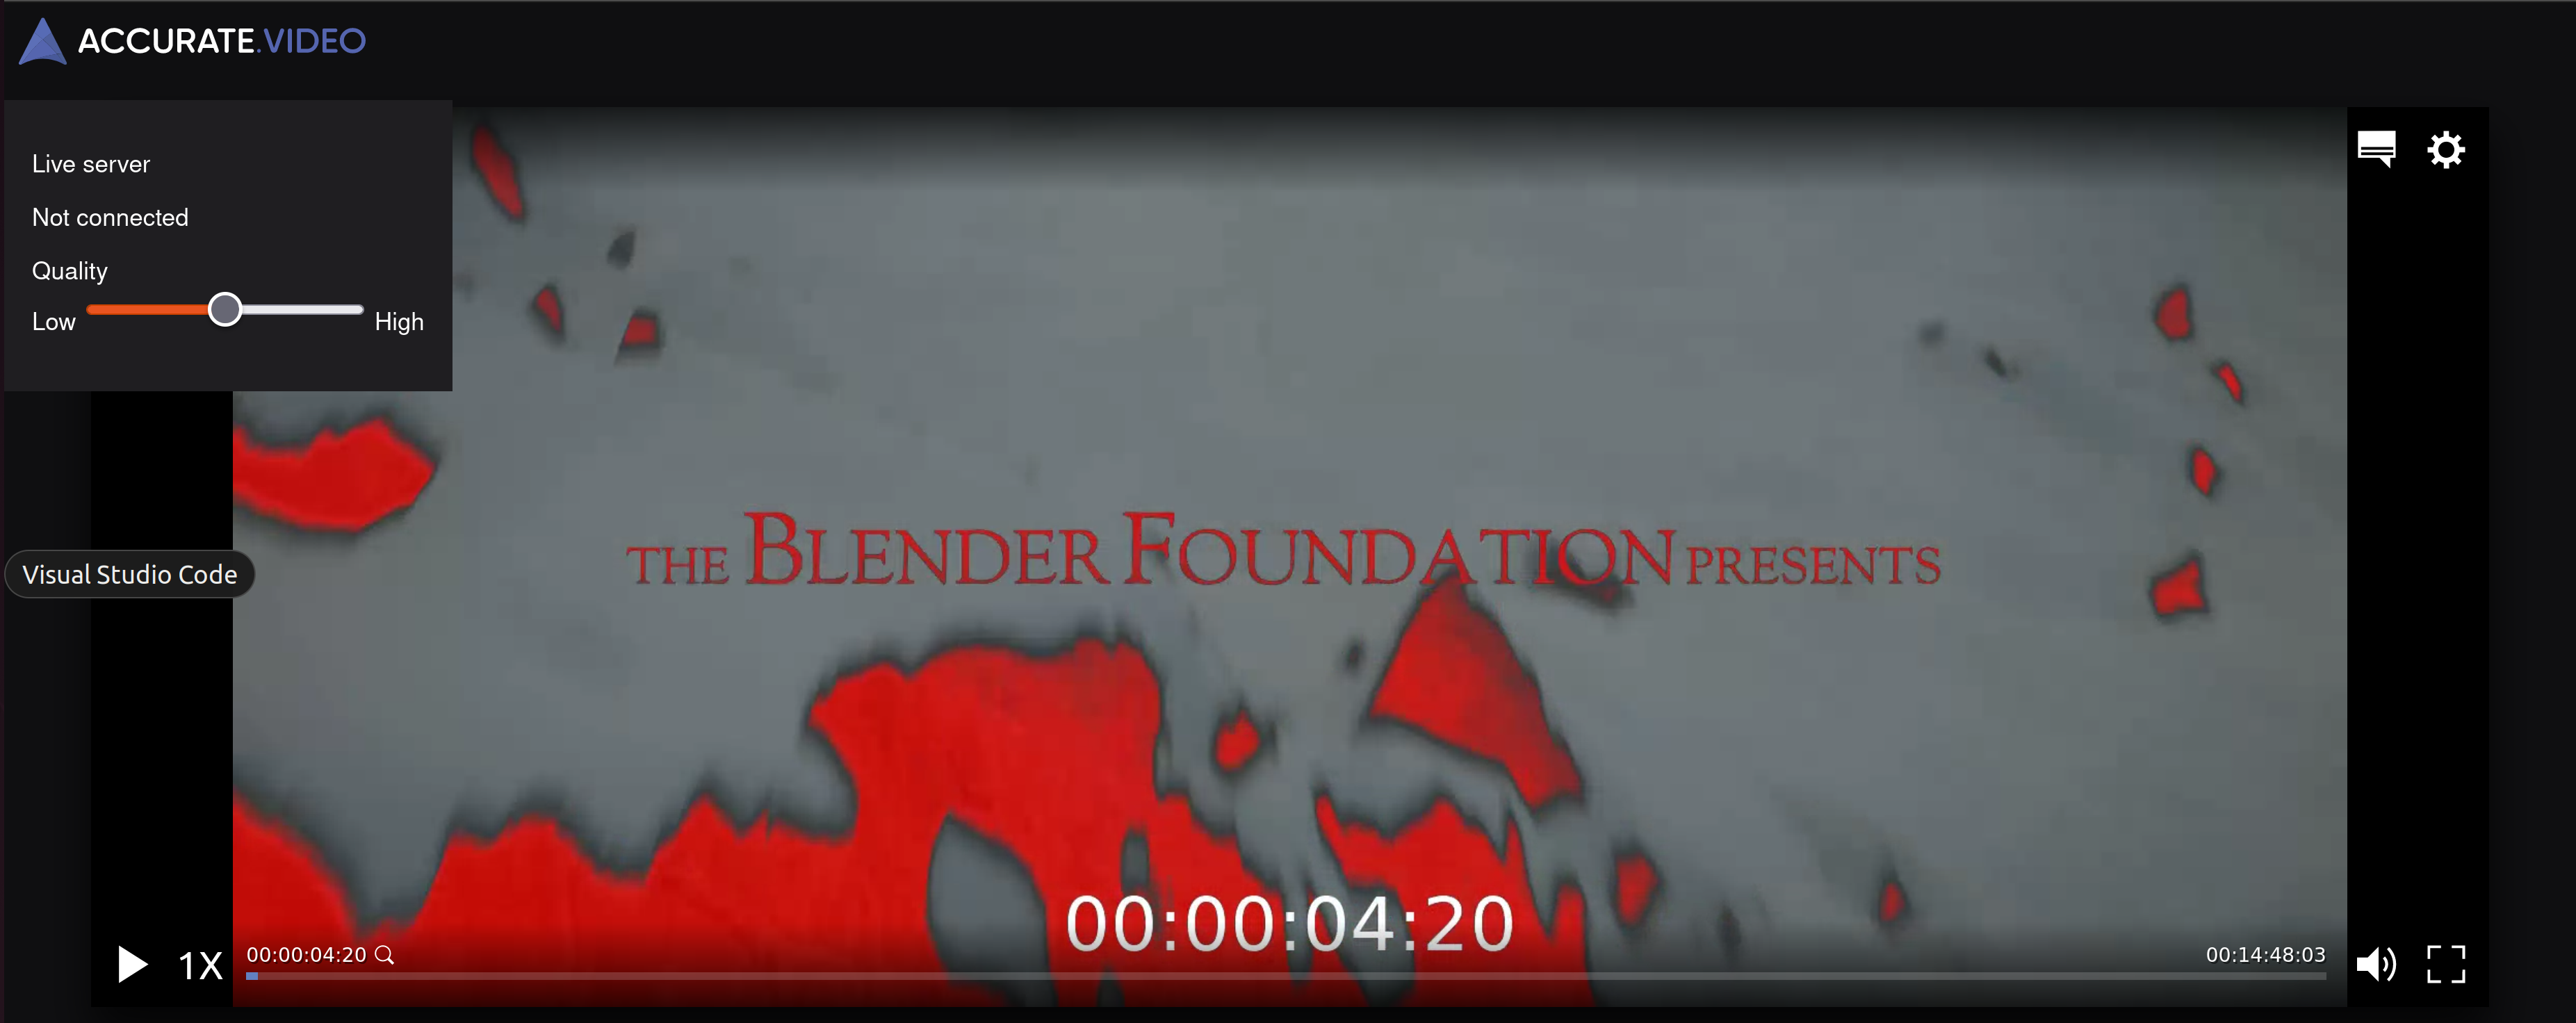
\includegraphics[width=0.8\textwidth]{ap_red.png}
%\end{center}


To compare the listed filters and their parameters, different values to change the red tones of the video will be tested and compared, assuming that the change of green and blue works analogous.

In addition to this, it needs to be tested, if multiple parameters of the same filter can be applied simultaneously. For evaluating, the filters and their different parameters for green and red are applied to the same frame of the test video file. This should result in a yellow output. 

Two frames with different colour schemes and content are used for those tests. One shows a snow landscape and the \textit{Blender Institute Production}-text and the other one shows an old man. The original frames $343$ and $3377$ can be seen in Figure~\ref{figure:nofilter}.

\begin{figure}[H]
	\begin{center}
		\cutpic{0.3cm}{0.45\textwidth}{nofilter_snow.png}
		\cutpic{0.3cm}{0.45\textwidth}{nofilter_man.png}
		\caption[Frames $343$ and $3377$ from the test video file without a filter.]{Frames $343$ on the left and $3377$ on the right from the test video file without a filter.}
		\label{figure:nofilter}
	\end{center}
\end{figure}

The filters were applied with the following CLI command:
\begin{lstlisting}[language=bash, numbers=none]
	melt -filter <filter_name> <filter_parameter> https://s3.eu-central-1.amazonaws.com/accurate-player-demo-assets/timecode/sintel-2048-timecode-stereo.mp4 -consumer xgl
\end{lstlisting}















%--------------------------------------------------------------------------------------
\subsubsection*{Filter \texttt{avfilter.colorbalance}}

The parameters of this filter take input values as float between $-1$ and $1$. It has individual parameters to set the shadows, mid tones and highlights per colour. This can be seen in Figure~\ref{figure:rs1rm1rh1}.

\begin{figure}[H]
	\begin{center}
		\cutpic{0.32cm}{0.3\textwidth}{rs_snow.png}
		%\hspace*{0.01\textwidth}
		\cutpic{0.32cm}{0.3\textwidth}{rm_snow.png}
		%\hspace*{0.01\textwidth}
		\cutpic{0.32cm}{0.3\textwidth}{rh_snow.png}
		% \small{
		%\texttt{av.rs=1} \hspace*{0.22\textwidth} \texttt{av.rm=1} \hspace*{0.23\textwidth} \texttt{av.rh=1}}
		\cutpic{0.32cm}{0.3\textwidth}{rs_man.png}
		%\hspace*{0.01\textwidth}
		\cutpic{0.32cm}{0.3\textwidth}{rm_man.png}
		%\hspace*{0.01\textwidth}
		\cutpic{0.32cm}{0.3\textwidth}{rh_man.png}
		\small{
		\texttt{av.rs=1} \hspace*{0.22\textwidth} \texttt{av.rm=1} \hspace*{0.23\textwidth} \texttt{av.rh=1}}
		\caption[Different parameters from the filter \texttt{avfilter.colorbalance} applied.]{Different parameters from the filter \texttt{avfilter.colorbalance} applied: Left with \texttt{av.rs=1} for red shadows, middle with \texttt{av.rm=1} for red mid tones and right with \texttt{av.rh=1} for red highlights.}
			\label{figure:rs1rm1rh1}
	\end{center}
\end{figure}

To get an even result of the colour on the frame, which would be applicable for the colour change with one slider. In Figure~\ref{figure:rsrmrh1}, the shadows, mid tones and highlights for the red value are set to $1$. 

\begin{figure}[H]
	\begin{center}
		\cutpic{0.3cm}{0.45\textwidth}{rsrmrh_snow.png}
		\cutpic{0.3cm}{0.45\textwidth}{rsrmrh_man.png}
		\label{figure:rsrmrh1}
		\caption[Parameters set to $1$ for red using the \texttt{avfilter.colorbalance} filter.]{All parameters for red with the value $1$  from the filter \texttt{avfilter.colorbalance} applied: \texttt{av.rs=1}, \texttt{av.rm=1} and \texttt{av.rh=1}.}
	\end{center}
\end{figure}

To evaluate if and how the overlay of different filters works, the values for green and red shadows, mid tones and highlights are set to $1$ and applied together. The parameters that are applied are \texttt{av.rs=1}, \texttt{av.rm=1}, \texttt{av.rh=1}, \texttt{av.gs=1}, \texttt{av.gm=1} and \texttt{av.gh=1}.
This results in yellow toned pictures.


\begin{figure}[H]
	\begin{center}
		\cutpic{0.3cm}{0.45\textwidth}{cb_yellow.png}
		\cutpic{0.3cm}{0.45\textwidth}{cb_yellow_man.png}
		\label{figure:cb_yellow}
		\caption[Red and green parameters set to $1$ with \texttt{avfilter.colorbalance}.]{All parameters for red and green with the value $1$  from the filter \texttt{avfilter.colorbalance} applied: \texttt{av.rs=1}, \texttt{av.rm=1}, \texttt{av.rh=1}, \texttt{av.gs=1}, \texttt{av.gm=1} and \texttt{av.gh=1}.}
	\end{center}
\end{figure}













%--------------------------------------------------------------------------------------

\subsubsection*{Filter \texttt{avfilter.colorchannelmixer}}

The parameters of this filter take input values as float between $-2$ and $2$. It has individual parameters to set the red, green, blue or alpha gain for the red, green, blue or alpha channel. The application of those parameters can be seen in Figure~\ref{figure:rrraar}.

\begin{figure}[H]
	\begin{center}
		\cutpic{0.32cm}{0.3\textwidth}{rr_snow.png}
		%\hspace*{0.01\textwidth}
		\cutpic{0.32cm}{0.3\textwidth}{ra_snow.png}
		%\hspace*{0.01\textwidth}
		\cutpic{0.32cm}{0.3\textwidth}{ar_snow.png}
		% \small{
			%\texttt{av.rs=1} \hspace*{0.22\textwidth} \texttt{av.rm=1} \hspace*{0.23\textwidth} \texttt{av.rh=1}}
		\cutpic{0.32cm}{0.3\textwidth}{rr_man.png}
		%\hspace*{0.01\textwidth}
		\cutpic{0.32cm}{0.3\textwidth}{ra_man.png}
		%\hspace*{0.01\textwidth}
		\cutpic{0.32cm}{0.3\textwidth}{ar_man.png}
		\small{
			\texttt{av.rr=2} \hspace*{0.22\textwidth} \texttt{av.ra=2} \hspace*{0.23\textwidth} \texttt{av.ar=2}}
		\caption[Different parameters from \texttt{avfilter.colorchannelmixer} applied.]{Different parameters from the filter \texttt{avfilter.colorchannelmixer} applied: Left with \texttt{av.rr=2} for red gain on the red channel, middle with \texttt{av.ra=2} for alpha gain on the red channel and right with \texttt{av.ar=2} for red gain on the alpha channel.}
		\label{figure:rrraar}
	\end{center}
\end{figure}


In Figure~\ref{figure:rrbrgr}, the red gain on the red, blue and green channel is applied. The parameter setting are \texttt{av.rr=2}, \texttt{av.gr=2} and \texttt{av.br=2}.


\begin{figure}[H]
	\begin{center}
		\cutpic{0.3cm}{0.45\textwidth}{rrbrgr_snow.png}
		\cutpic{0.3cm}{0.45\textwidth}{rrbrgr_man.png}
		\label{figure:rrbrgr}
		\caption[Red gain set to $2$ with \texttt{avfilter.colorchannelmixer}.]{Red gain with the value $2$ for the red, green and blue channel from the filter \texttt{avfilter.colorchannelmixer} applied: \texttt{av.rr=2}, \texttt{av.gr=2} and \texttt{av.br=2}.}
	\end{center}
\end{figure}


To evaluate if and how the overlay of different filters works, the values for the green and red gain on the green and red channel are set to $2$ and applied together. The parameters that are applied are \texttt{av.rr=2} and \texttt{av.gg=2}. This results in yellow toned pictures.


\begin{figure}[H]
	\begin{center}
		\cutpic{0.3cm}{0.45\textwidth}{rrgg_snow.png}
		\cutpic{0.3cm}{0.45\textwidth}{rrgg_man.png}
		\label{figure:rrgg}
		\caption[Red and green gain set to $2$ with \texttt{avfilter.colorchannelmixer}.]{Red and green gain on the red and green channel with the value $2$ from the filter \texttt{avfilter.colorchannelmixer} applied: \texttt{av.rr=2} and \texttt{av.gg=2}.}
	\end{center}
\end{figure}







%--------------------------------------------------------------------------------------
\subsubsection*{Filter \texttt{frei0r.coloradj\_RGB}}

The parameters of this filter take input values as float between $0$ and $1$. It has individual parameters to set the red, green, blue value. The application of the red parameters can be seen in Figure~\ref{figure:r}.


\begin{figure}[H]
	\begin{center}
		\cutpic{0.3cm}{0.45\textwidth}{r_snow.png}
		\cutpic{0.3cm}{0.45\textwidth}{r_man.png}
		\label{figure:r}
		\caption[Red parameter set to $1$ with \texttt{frei0r.coloradj\_RGB}.]{Red parameter with the value $1$ from the filter \texttt{frei0r.coloradj\_RGB} applied: \texttt{R=1}.}
	\end{center}
\end{figure}



To evaluate if and how the overlay of different filters works, the values for the green and red parameter are set to $1$ and applied together. The parameters that are applied are \texttt{R=1} and \texttt{G=1}. This results in yellow toned pictures, which can be seen in Figure~\ref{figure:rg}.


\begin{figure}[H]
	\begin{center}
		\cutpic{0.3cm}{0.45\textwidth}{rg_snow.png}
		\cutpic{0.3cm}{0.45\textwidth}{rg_man.png}
		\label{figure:rg}
		\caption[Red and green parameter set to $1$ with \texttt{frei0r.coloradj\_RGB}.]{Red and green parameter with the value $1$ from the filter \texttt{frei0r.coloradj\_RGB} applied: \texttt{R=1} and \texttt{G=1}.}
	\end{center}
\end{figure}




\subsubsection*{Evaluation}

%the filters are compared regarding the result of the application of one flter and for this the vibrance and intensity is the important factor and regarding the mixing of colours and here vibrance and intensity are the important aspects as well



The Melt filters \texttt{avfilter.colorbalance}, \texttt{avfilter\-.colorchannelmixer} and \texttt{frei\-0r\-.coloradj\_RGB} are compared regarding the colour vibrance and intensity of the result. This regards the colour intensity of a single colour value change (red, green and blue) and mixed colurs.

% For the comparison of the result of the single colour filter application, the following parameters per filter are chosen:

In the following, the results of the change of a single colour (red) for each of the filters can be seen:

\begin{figure}[H]
	\centering
	\begin{tabular}{c|c|c}
		
		\footnotesize{\texttt{avfilter.colorbalance}} & \footnotesize{\texttt{avfilter.colorchannelmixer}} & \footnotesize{\texttt{frei0r.coloradj\_RGB}} \\
		
		\scriptsize{\texttt{av.rs=1} \texttt{av.rm=1} \texttt{av.rh=1}} & \scriptsize{\texttt{av.rr=2}} & \scriptsize{\texttt{R=1}} \\
		
		\cutpic{0.3cm}{0.29\textwidth}{rsrmrh_snow.png} & \cutpic{0.3cm}{0.29\textwidth}{rr_snow.png} & \cutpic{0.3cm}{0.29\textwidth}{r_snow.png} \\
		
		\cutpic{0.3cm}{0.29\textwidth}{rsrmrh_man.png} & \cutpic{0.3cm}{0.29\textwidth}{rr_man.png} & \cutpic{0.3cm}{0.29\textwidth}{r_man.png} \\
		
	\end{tabular}
	
	\caption{Comparison of red filter option of all three filters.}
	\label{figure:redcomp}

\end{figure}

In Figure~\ref{figure:redcomp} can be seen, that the colour of the \texttt{avfilter.colorbalance} is the most intense and vibrant. This leads to a broader colour range and more options for personalisation.




In the following, the results of the application of two mixed colours for each of the filters can be seen. The chosen colours are red and green, whch should lead to a yellow result.

\begin{figure}[H]
	\centering
	\begin{tabular}{c|c|c}
		
		\footnotesize{\texttt{avfilter.colorbalance}} & \footnotesize{\texttt{avfilter.colorchannelmixer}} & \footnotesize{\texttt{frei0r.coloradj\_RGB}} \\
		
		\scriptsize{\texttt{av.rs=1} \texttt{av.rm=1} \texttt{av.rh=1}} & \scriptsize{\texttt{av.rr=2}}  & \scriptsize{\texttt{R=1}} \\
		\scriptsize{\texttt{av.gs=1} \texttt{av.gm=1} \texttt{av.gh=1}} & \scriptsize{\texttt{av.gg=2}}  & \scriptsize{\texttt{G=1}} \\
		
		\cutpic{0.3cm}{0.29\textwidth}{cb_yellow.png} & \cutpic{0.3cm}{0.29\textwidth}{rrgg_snow.png} & \cutpic{0.3cm}{0.29\textwidth}{rg_snow.png} \\
		
		\cutpic{0.3cm}{0.29\textwidth}{cb_yellow_man.png} & \cutpic{0.3cm}{0.29\textwidth}{rrgg_man.png} & \cutpic{0.3cm}{0.29\textwidth}{rg_man.png} \\
		
	\end{tabular}
	
	\caption{Comparison of red filter option of all three filters.}
	\label{figure:yellowcomp}
	
\end{figure}

In Figure~\ref{figure:yellowcomp} can be seen, that the colour of the \texttt{avfilter.colorbalance} is the most intense and vibrant again. This leads to a broader colour range and more options for personalisation.

In the above shown cases cases, the results of the \texttt{avfilter.colorchannelmixer} filter have more depth and look more dynamic, because the colour gain was only executed on the corresponding colour channels. This might be an aspect, that lets the user achieve more aesthetically pleasing results but the overall intensity of the colours is lower. In addition to this, the expected behaviour of a slider for the RGB colour change might not be to only change the colour intensity on one colour channel. Based on this, the filter \texttt{avfilter.colorbalance} seems to deliver the most fitting results in those criteria.




The \texttt{avfilter.colorbalance} filter leads to the most vibrant and intense results of the above listed selection of filters. Additionally it has the option to adapt the shadows, mid tones and highlights individually, which creates the option for more (pre)adjustment of the results in the backend and introducing more sliders or options for the user for adjustment as future work.
But on the downside, to tone the whole frame, three instead of one parameter have to be applied -- for the shadows, mid tones and highlights.
When applying this with and without JIT, no performance difference was noticeable but for a accurate evaluation of this, performance tests would have to be performed and the implementations of the filters would need to be examined.

Examining and evaluating the different options of the Melt filters is an interesting option for future work or for Codemill to implement. For this thesis project, the filter \texttt{avfilter.colorbalance} will be used, because it results look the most vibrant.

In Figure~\ref{figure:septopus}, the 7 colour combinations of the subtractive colour model can be seen as the application of the filter \texttt{avfilter.colorbalance}. for this, the RGB values were either set to $1.0$ or $0$, which are the maximum and default values of this filter. 



\begin{figure}[H]
	\begin{center}
		\cutpic{0.3cm}{0.8\textwidth}{septopus.png}
		\label{figure:septopus}
		\caption[Base colours with the application of the filter \texttt{avfilter.colorbalance}.]{Base colours of the subtractive colour model with the application of the filter \texttt{avfilter.colorbalance}.}
	\end{center}
\end{figure}

The original frame is frame 3447 from the test video file and can be seen in Figure~\ref{figure:septo_nofilter}.

\begin{figure}[H]
	\begin{center}
		\cutpic{0.3cm}{0.4\textwidth}{septopus_nofilter.png}
		\label{figure:septo_nofilter}
		\caption[Frame 3447 of the test video file without a filter.]{Frame 3447 of the test video file without a filter.}
	\end{center}
\end{figure}












% \newpage
%-------------------------------------------------------------------------------------------------------
\subsection{Implementation} \label{subsection:implementation}
% Discuss the technologies and tools chosen for the implementation.

In this Section, the implementation is described. This is separated into three parts, that are described individually: Frontend, proto buffer and the application of the filter in the backend.

%-----------------------------------------------------------------------------------------------------------
\subsubsection*{Frontend}
%
\vspace*{-1em}
\begin{minipage}{0.48\textwidth}
In the frontend, input sliders for the user sided adjustment of the RGB values were added below the already existing slider for the quality adjustment. This is located in the overlay windows in the top right corner. The sliders were coloured according to their associated functions in red, green and blue. This can be seen in Figure~\ref{figure:sliders}.

The HTML code for the red slider can be seen below. The other sliders for green and blue work analogical. The input range is set between $-100$ and $100$, to divide it later by $100$ to achieve a float 




\end{minipage}\begin{minipage}{0.04\textwidth}
\ 
\end{minipage}\begin{minipage}{0.48\textwidth}
\begin{figure}[H]
	\begin{center}
		\cutpic{0.3cm}{0.9\textwidth}{sliders.png}
		\caption[Sliders for RGB colour adjustment.]{Sliders for RGB colour adjustment.}
		\label{figure:sliders}
	\end{center}
\end{figure}
\hfill
\end{minipage}

\vspace*{-1.3em}
value between $-1$ and $1$ for the filter parameter. The default value is set to $0$. The input value from the slider then gets read out in a TypeScript file.  


\begin{lstlisting}[language=html, numbers=none]
	<p>
		<label for="red-slider">Red</label><br />
		Low
		<input
			type="range"
			min="-100"
			max="100"
			value="0"
			class="slider"
			id="red-slider"
		/>
		High
	</p>
\end{lstlisting}






%-----------------------------------------------------------------------------------------------------------
\subsubsection*{Proto Buffer}

For the data transfer between frontend and backend for the colour grading, fields and enums were added to the \texttt{.proto} file. Proto buffers are explained in Section~\ref{subsection:protocolbuffer}. The 
%
\begin{minipage}{0.54\textwidth}
\vspace*{-0.2em}
\begin{lstlisting}[style=protobufStyle, numbers=none]
syntax = "proto2";
	
message JitControl {
	...
	optional float red_value = 4;  
	optional float green_value = 5; 
	optional float blue_value = 6; 
}
	
enum ControlType {
	...
	RED_VALUE = 7;
	GREEN_VALUE = 8;
	BLUE_VALUE = 9;
}
\end{lstlisting}
\hfill
\end{minipage}\begin{minipage}{0.04\textwidth}
	\ 
\end{minipage}\begin{minipage}{0.42\textwidth}
\vspace*{0.7em}
values that were retrieved by the previously described sliders for the RGB value are transferred with this data structure.
In the code, the message \texttt{JitControl} and the enum \texttt{ControlType} can be seen. 
In the message, three optional fields for the red, green and blue value are defined as \texttt{red\_value}, \texttt{green\_value} and \texttt{blue\_value} to represent the RGB colour values. 
In the enum, the three constants (\texttt{RED\_VALUE}, \texttt{GREEN\_VALUE}, and \texttt{BLUE\_VALUE}) were added. 
Through the sliders in the frontend, users can manipulate these values for red, green

\end{minipage}

and blue. The input values of those sliders are read out and assigned to the enum \texttt{JITAction} in the frontend. They are then transmitted to the backend with the proto2 data format. The application of the Melt filters with the retrieved values is described in the following part.











%-----------------------------------------------------------------------------------------------------------
\subsubsection*{Application of the Melt filter}


\begin{minipage}{0.60\textwidth}
	The application of the Melt filter is implemented in the \texttt{jit.c} file. To be bale to apply multiple values for the three different colour channels at once, the command needs to be sent to Melt with all of the 
\end{minipage}\begin{minipage}{0.04\textwidth}
	\ 
\end{minipage}\begin{minipage}{0.36\textwidth}
	{\tiny\begin{lstlisting}[language=c, numbers=none]
		float red_value;
		float green_value;
		float blue_value; \end{lstlisting}}
	\vfill
\end{minipage}

according parameters set, else the other parameters will be overwritten with the default value $0$. To be able to achieve mixed colour results, including for example yellow, the previous values need to be sent to the Melt framework together with the changed value. This is implemented with initializing global variables for each of the colours, that are set to the current value in each call. This can be seen in the code snippet above.

The appilcation of the Melt filter with the current input values from the sliders is implemented in the function \texttt{jit\_action()}, that has a Melt producer as a parameter. In the following code, the beginning of the function can be seen. The Melt properties, consumer and producer are retrieved and set. Then the filter \texttt{avfilter.colorbalance} is set. The comparison of the different filter options can be seen in Section~\ref{subsection:meltfilter}.


\begin{lstlisting}[language=c, numbers=none, columns=fullflexible]	
mlt_properties properties = MLT_PRODUCER_PROPERTIES(producer);
mlt_consumer consumer = mlt_properties_get_data(properties, "transport_consumer", NULL);
...	
mlt_producer service = mlt_producer_service(producer);
mlt_filter filter = mlt_factory_filter(service, "avfilter.colorbalance", NULL);	
\end{lstlisting}


In the following, a pointer \texttt{jit\_control} is declared, that casts a value into the type \texttt{JitControl}.
Then, a switch statement is started, based on the value of \texttt{jit\_control}.
The \texttt{->} operator is used to access the type field of the \texttt{jit\_control} structure and depending on the value, the execution will jump to the corresponding case within the switch statement.

\begin{lstlisting}[language=c, numbers=none, columns=fullflexible]		
JitControl *const jit_control = (JitControl*) value;
switch (jit_control->type) { ...
\end{lstlisting}

Three cases were implemented -- one for each colour value (red, green, blue). In the following, the switch case for the adjustment of the red value is explained in more detail. The other cases work analogical.

In the following code, the case for the red value can be seen. First, the red value that was retrieved from the slider in the frontend is assigned to the variable \texttt{red\_value}. Then, an \texttt{mlt\_properties} object is created for setting the filter parameters later on. 

\begin{lstlisting}[language=c, numbers=none, columns=fullflexible]			
case CONTROL_TYPE__RED_VALUE:
	red_value = jit_control->red_value;
	{
		mlt_properties filter_props_red = mlt_filter_properties(filter);
\end{lstlisting}

In the first if statement of this case, the red value is added to the filter properties. For this, it gets checked if the value is in the input range of the filter parameter. Then, a string containing the value is created, because the function \texttt{mlt\_properties\_set} requires the value for the filter parameter in string format. After this, the filter properties are set to this value. Three parameters per colour have to be set, because the chosen filter has the possibility of adjusting the shadows, mid tones and highlights individually. 
The comparison of the different filters can be seen in Section~\ref{subsection:meltfilter} and the described code can be seen below.


\begin{lstlisting}[language=c, numbers=none, columns=fullflexible]
		if (red_value >= -1.0 && red_value <= 1.0) {
			char red_value_str[20]; 
			snprintf(red_value_str, sizeof(red_value_str), "%.2f", red_value);
			mlt_properties_set(filter_props_red, "av.rs", red_value_str);
			mlt_properties_set(filter_props_red, "av.rm", red_value_str);
			mlt_properties_set(filter_props_red, "av.rh", red_value_str);
		}	
\end{lstlisting}

The previous values for the green and red values were saved in the variables, that were declared outside of the function. In the following, the values are set analogical to the above described red value. This is neccessary to not overwrite the previously adjusted colour values.
	
\begin{lstlisting}[language=c, numbers=none, columns=fullflexible]
		if (green_value >= -1.0 && green_value <= 1.0) {
			char green_value_str[20]; 
			snprintf(green_value_str, sizeof(green_value_str), "%.2f", green_value);
			mlt_properties_set(filter_props_red, "av.gs", green_value_str);
			mlt_properties_set(filter_props_red, "av.gm", green_value_str);	
			mlt_properties_set(filter_props_red, "av.gh", green_value_str);
		} 			
		if (blue_value >= -1.0 && blue_value <= 1.0) {
			char blue_value_str[20]; 
			snprintf(blue_value_str, sizeof(blue_value_str), "%.2f", blue_value);
			mlt_properties_set(filter_props_red, "av.bs", blue_value_str);
			mlt_properties_set(filter_props_red, "av.bm", blue_value_str);	
			mlt_properties_set(filter_props_red, "av.hs", blue_value_str);
		}					
	}
\end{lstlisting}

In the following code snippet, the filter and the producer get connected and then the consumer and the filter get connected aswell.


\begin{lstlisting}[language=c, numbers=none, columns=fullflexible]
	mlt_filter_connect(filter, service, 0);
	mlt_consumer_connect(consumer, mlt_filter_service(filter));
	break;			
\end{lstlisting}

This case shows the code that is executed, when the slider for the red value is changed in the frontend and the red value is applied to the video output in real time with the Melt framework.

The implementation of the switch case for the green value can be seen in the following:

\begin{lstlisting}[language=c, numbers=none, columns=fullflexible]
case CONTROL_TYPE__GREEN_VALUE:
green_value = jit_control->green_value;
{
	mlt_properties filter_props_green = mlt_filter_properties(filter);
	
	if (red_value >= -1.0 && red_value <= 1.0) {
		char red_value_str[20]; 
		snprintf(red_value_str, sizeof(red_value_str), "%.2f", red_value);
		mlt_properties_set(filter_props_green, "av.rs", red_value_str);
		mlt_properties_set(filter_props_green, "av.rm", red_value_str);
		mlt_properties_set(filter_props_green, "av.rh", red_value_str);
	}	
	if (green_value >= -1.0 && green_value <= 1.0) {
		char green_value_str[20]; 
		snprintf(green_value_str, sizeof(green_value_str), "%.2f", green_value);
		mlt_properties_set(filter_props_green, "av.gs", green_value_str);
		mlt_properties_set(filter_props_green, "av.gm", green_value_str);
		mlt_properties_set(filter_props_green, "av.gh", green_value_str);
	}		
	if (blue_value >= -1.0 && blue_value <= 1.0) {
		char blue_value_str[20]; 
		snprintf(blue_value_str, sizeof(blue_value_str), "%.2f", blue_value);
		mlt_properties_set(filter_props_green, "av.bs", blue_value_str);
		mlt_properties_set(filter_props_green, "av.bm", blue_value_str);
		mlt_properties_set(filter_props_green, "av.hs", blue_value_str);
	}		
}	
	mlt_filter_connect(filter, service, 0);
	mlt_consumer_connect(consumer, mlt_filter_service(filter));
	break;

\end{lstlisting}

The implementation of the switch case for the blue value can be seen in the following:

\begin{lstlisting}[language=c, numbers=none, columns=fullflexible]	
case CONTROL_TYPE__BLUE_VALUE:
	blue_value = jit_control->blue_value;
	{
		mlt_properties filter_props_blue = mlt_filter_properties(filter);
		
		if (red_value >= -1.0 && red_value <= 1.0) {
			char red_value_str[20]; 
			snprintf(red_value_str, sizeof(red_value_str), "%.2f", red_value);
			mlt_properties_set(filter_props_blue, "av.rs", red_value_str);
			mlt_properties_set(filter_props_blue, "av.rm", red_value_str);
			mlt_properties_set(filter_props_blue, "av.rh", red_value_str);
		}	
		if (green_value >= -1.0 && green_value <= 1.0) {
			char green_value_str[20]; 
			snprintf(green_value_str, sizeof(green_value_str), "%.2f", green_value);
			mlt_properties_set(filter_props_blue, "av.gs", green_value_str);
			mlt_properties_set(filter_props_blue, "av.gm", green_value_str);
			mlt_properties_set(filter_props_blue, "av.gh", green_value_str);
		}	
		if (blue_value >= -1.0 && blue_value <= 1.0) {
			char blue_value_str[20]; 
			snprintf(blue_value_str, sizeof(blue_value_str), "%.2f", blue_value);
			mlt_properties_set(filter_props_blue, "av.bs", blue_value_str);
			mlt_properties_set(filter_props_blue, "av.bm", blue_value_str);
			mlt_properties_set(filter_props_blue, "av.hs", blue_value_str);
		}	
	}
	mlt_filter_connect(filter, service, 0);
	mlt_consumer_connect(consumer, mlt_filter_service(filter));
	break;  

\end{lstlisting}



	
	
	
\end{document}